% Festlegung des Allgemeinen Dokumentenformats
\documentclass[a4paper,12pt,headsepline]{scrartcl}

% Umlaute unter UTF8 nutzen
\usepackage[utf8]{inputenc}

% Variablen
%Variablen welche innerhalb der gesamten Arbeit zur Verfügung stehen sollen
\newcommand{\titleDocument}{Bachelorarbeit}
\newcommand{\subjectDocument}{
    Analyse der Echtzeitfähigkeit von Micro-ROS und FreeRTOS am Beispiel einer
    Robotersteuerungssoftware
}


% weitere Pakete
% Grafiken aus PNG Dateien einbinden
\usepackage{graphicx}
\usepackage{tikz}

% Deutsche Sonderzeichen und Silbentrennung nutzen
\usepackage[ngerman]{babel}

% Eurozeichen einbinden
\usepackage[right]{eurosym}

% Zeichenencoding
\usepackage[T1]{fontenc}

\usepackage{lmodern}

% floatende Bilder ermöglichen
%\usepackage{floatflt}

\usepackage{float}

% mehrseitige Tabellen ermöglichen
\usepackage{longtable}

\usepackage{diagbox}
\usepackage{colortbl}

% Unterstützung für Schriftarten
%\newcommand{\changefont}[3]{ 
%\fontfamily{#1} \fontseries{#2} \fontshape{#3} \selectfont}

% Packet für Seitenrandabständex und Einstellung für Seitenränder
\usepackage{geometry}
\geometry{left=3.5cm, right=2cm, top=2.5cm, bottom=2cm}

% Paket für Boxen im Text
\usepackage{fancybox}

% bricht lange URLs "schön" um
\usepackage[hyphens,obeyspaces,spaces]{url}

% Paket für Textfarben
\usepackage{color}

% Mathematische Symbole importieren
\usepackage{amssymb}

\usepackage{amsmath}

% auf jeder Seite eine Überschrift (alt, zentriert)
%\pagestyle{headings}

\usepackage{pdfpages}

% erzeugt Inhaltsverzeichnis mit Querverweisen zu den Abschnitten (PDF Version)
\usepackage[bookmarksnumbered,pdftitle={\titleDocument},hyperfootnotes=false]{hyperref}
%\hypersetup{colorlinks, citecolor=red, linkcolor=blue, urlcolor=black}
%\hypersetup{colorlinks, citecolor=black, linkcolor= black, urlcolor=black}

% neue Kopfzeilen mit fancypaket
\usepackage{fancyhdr} %Paket laden
\pagestyle{fancy} %eigener Seitenstil
\fancyhf{} %alle Kopf- und Fußzeilenfelder bereinigen
\fancyhead[L]{\nouppercase{\leftmark}} %Kopfzeile links
\fancyhead[C]{} %zentrierte Kopfzeile
\fancyhead[R]{\thepage} %Kopfzeile rechts
\renewcommand{\headrulewidth}{0.4pt} %obere Trennlinie
%\fancyfoot[C]{\thepage} %Seitennummer
%\renewcommand{\footrulewidth}{0.4pt} %untere Trennlinie

% change font to serif for headings - buggy
% \usepackage{sectsty}
% \allsectionsfont{\normalfont\bfseries}

% für Tabellen
\usepackage{array}

% Runde Klammern für Zitate
%\usepackage[numbers,round]{natbib}

% Festlegung Art der Zitierung - Havardmethode: Abkuerzung Autor + Jahr
\bibliographystyle{alphadin}

% Schaltet den zusätzlichen Zwischenraum ab, den LaTeX normalerweise nach einem Satzzeichen einfügt.
%\frenchspacing

% Paket für Zeilenabstand
\usepackage{setspace}

% für Bildbezeichner
\usepackage{capt-of}

% für Stichwortverzeichnis
\usepackage{makeidx}

%Konfiguriere das Inhaltsverzeichnis
\usepackage{tocbasic}
\DeclareTOCStyleEntries[
  raggedentrytext,
  numwidth=0pt,
  numsep=1ex,
  dynnumwidth,
]{tocline}{chapter,section,subsection,subsubsection,paragraph,subparagraph}
\DeclareTOCStyleEntries[
  indent=0pt,
  linefill=\TOCLineLeaderFill,
]{tocline}{section,subsection,subsubsection,paragraph,subparagraph}


% für Listings
% \usepackage{listings}
% \lstset{numbers=left, numberstyle=\tiny, numbersep=5pt, keywordstyle=\color{black}\bfseries, stringstyle=\ttfamily,showstringspaces=false,basicstyle=\footnotesize,captionpos=b}
\usepackage{xcolor}
\usepackage[newfloat]{minted}
\usepackage{caption}
\usepackage{fancyhdr}
\newenvironment{code}{\captionsetup{type=listing}}{}
\SetupFloatingEnvironment{listing}{name=Quellcode}
\setminted{
    linenos,
    frame=single,
    bgcolor=black!5,
    fontsize=\footnotesize
}
\usepackage{graphicx}  % Add this to your preamble

\usepackage[withpage]{acronym}

% Absatz ohne Einrückung
\setlength{\parskip}{1em} % 1em entspricht der Breite eines 'M'-Zeichens
\setlength{\parindent}{0pt}

% Indexerstellung
\makeindex

% Abkürzungsverzeichnis
\usepackage[german]{nomencl}
\let\abbrev\nomenclature

% Abkürzungsverzeichnis LiveTex Version
% Titel des Abkürzungsverzeichnisses
\renewcommand{\nomname}{Abkürzungsverzeichnis}
% Abstand zwischen Abkürzung und Erläuterung
\setlength{\nomlabelwidth}{.25\textwidth}
% Zwischenraum zwischen Abkürzung und Erläuterung mit Punkten
\renewcommand{\nomlabel}[1]{#1 \dotfill}
% Variation des Abstandes der einzelnen Abkürzungen zu einander
\setlength{\nomitemsep}{-\parsep}
% Index mit Abkürzungen erzeugen
\makenomenclature
%\makeglossary

% Abkürzungsverzeichnis TeTEX Version
% \usepackage[german]{nomencl}
% \makenomenclature
% %\makeglossary
% \renewcommand{\nomname}{Abkürzungsverzeichnis}
% \AtBeginDocument{\setlength{\nomlabelwidth}{.25\columnwidth}}
% \renewcommand{\nomlabel}[1]{#1 \dotfill}
% \setlength{\nomitemsep}{-\parsep}

% Optional: Einzelne Zeilen am Anfang einer Seite unterdrücken (Schusterjungen)
% \clubpenalty = 10000
% Optional: Einzelne Zeilen am Ende einer Seite unterdrücken (Hurenkinder)
% \widowpenalty = 10000
% \displaywidowpenalty = 10000

\begin{document}
% hier werden die Trennvorschläge inkludiert
%hier müssen alle Wörter rein, welche Latex von sich auch nicht korrekt trennt bzw. bei denen man die genaue Trennung vorgeben möchte
\hyphenation{
Film-pro-du-zen-ten
Lux-em-burg
Soft-ware-bau-steins
zeit-in-ten-siv
}


% Schriftart Helvetica verwenden
%\usepackage{helvet}
%\renewcommand\familydefault{\sfdefault}

% Leere Seite am Anfang
%\thispagestyle{empty} % erzeugt Seite ohne Kopf- / Fusszeile
%\mbox{}
%\newpage

% Titelseite %
\thispagestyle{empty}

% % Logo
% \begin{figure}[t]
%  \centering
%  
\includegraphics[width=0.3\textwidth]{assets/fhlogo.pdf}
% \end{figure}

\begin{center}
\textbf{\Large{~\titleDocument}}
\end{center}
\begin{verbatim}





\end{verbatim}
\begin{center}
\doublespacing
\textbf{\LARGE{\subjectDocument}}\\
\singlespacing
\end{center}
\begin{verbatim}
















\end{verbatim}
\begin{center}
\textbf{
    An der Fachhochschule Dortmund \\
    im Fachbereich Informatik \\
    Studiengang Technische Informatik \\
    erstellte Thesis \\
    zur Erlangung des akademischen Grades \\
    Bachelor of Science \\
    B. Sc. \\
}
\end{center}
\begin{center}
    \textbf{Xu, Zijian \linebreak
    geboren am 25.09.1998 \linebreak
    7204211
    }
\end{center}
\begin{flushleft}
\begin{tabular}{llll}
\textbf{Betreuung durch:} & & Prof. Dr. Christof Röhrig &\\
    & & M. Sc. Alexander Miller &\\
\textbf{Version vom:} & & Dortmund, \today &\\
\end{tabular}
\end{flushleft}


% römische Numerierung
\pagenumbering{Roman}

% 1.5 facher Zeilenabstand
\onehalfspacing

\newpage

% Einleitung / Abstract
\thispagestyle{empty}
\section*{Kurzfassung}

Diese Arbeit analysiert die Echtzeitfähigkeit von Micro-ROS und FreeRTOS anhand
einer Robotersteuerungssoftware. Ziel ist der Vergleich beider Systeme
hinsichtlich ihres Echtzeitverhaltens mit Schwerpunkt auf den Ausführungszeiten.
Dazu wird zunächst die bestehende Micro-ROS-Steuerungssoftware auf FreeRTOS
portiert. Anschließend wird eine zyklengenaue Messmethode für den Programmlauf
basierend auf der Data Watchpoint and Trace Unit (DWT) der ARM-Architektur
entwickelt. Zum Abschluss werden die Laufzeitdaten visualisiert und ausgewertet.
Die Ergebnisse verdeutlichen die unterschiedlichen Schwerpunkte beider
Plattformen: Micro-ROS punktet durch die Kompatibilität mit dem ROS-Ökosystem,
während FreeRTOS mit minimalen Latenzen und deterministischem Scheduling
deutlich besseres Echtzeitverhalten bietet. Die Analyse bestätigt zudem den
maßgeblichen Einfluss der Cache-Nutzung auf die Rechenleistung.

\section*{Abstract}

This thesis analyzes the real-time capabilities of micro-ROS and FreeRTOS using
a robotic control software. The goal is to compare both systems regarding their
real-time behavior emphasized on the execution times. First, the existing
micro-ROS control software is ported to FreeRTOS. Next, a cycle-accurate
measurement method for program execution based on ARM's Data Watchpoint and
Trace Unit (DWT)is developed. Finally, the runtime data is evaluated. The
evaluation of the results highlights the different strengths of both platforms:
micro-ROS stands out due to its compatibility with the ROS ecosystem, while
FreeRTOS achieves superior real-time behavior through minimal latencies and
deterministic scheduling. Additionally, the analysis confirms the significant
impact of the cache utilization on system performance.


% einfacher Zeilenabstand
\singlespacing

\newpage
% Seitenzählung bei Inhaltsverzeichnis beginnen
\setcounter{page}{1}

% Inhaltsverzeichnis anzeigen
\thispagestyle{empty}
\tableofcontents

\newpage
% das Abbildungsverzeichnis
% Verion 1: Abbildungsverzeichnis MIT führender Nummberierung endgueltig anzeigen
\listoffigures
% Abbildungsverzeichnis soll im Inhaltsverzeichnis auftauchen
\addcontentsline{toc}{section}{Abbildungsverzeichnis}

% Verion 2: Abbildungsverzeichnis OHNE führende Nummberierung endgueltig anzeigen
%\begingroup
%\renewcommand\numberline[1]{}
%\listoffigures
%\endgroup


% das Tabellenverzeichnis
\newpage
% \fancyhead[L]{Abbildungsverzeichnis / Abkürzungsverzeichnis} %Kopfzeile links
% Tabellenverzeichnis endgültig anzeigen
\listoftables
% Tabellenverzeichnis soll im Inhaltsverzeichnis auftauchen
\addcontentsline{toc}{section}{Tabellenverzeichnis}

% das Quellcodeverzeichnis
\newpage
\renewcommand*{\listlistingname}{Quellcodeverzeichnis}
\listoflistings % Add Quellcodeverzeichnis
\addcontentsline{toc}{section}{Quellcodeverzeichnis}

% das Abkürzungsverzeichnis
\newpage
% das Abkürzungsverzeichnis ausgeben
\fancyhead[L]{Abkürzungsverzeichnis} %Kopfzeile links
\section*{Abkürzungsverzeichnis}

\begin{acronym}
\end{acronym}

% \printnomenclature[3cm]
% Abkürzungsverzeichnis soll im Inhaltsverzeichnis auftauchen
\addcontentsline{toc}{section}{Abkürzungsverzeichnis}


%%%%%%% EINLEITUNG %%%%%%%%%%%%
\newpage
\fancyhead[L]{\nouppercase{\leftmark}} %Kopfzeile links

% 1,5 facher Zeilenabstand
\onehalfspacing

% arabische Seitennummerierung ab hier
\pagenumbering{arabic}

% Alternative Einbindung des Abstract in Kapitel "0" falls gewünscht
%\setcounter{section}{-1}
%\setcounter{page}{0}

% Option: Einbindung abstract
%\section*{Kurzfassung}

Diese Arbeit analysiert die Echtzeitfähigkeit von Micro-ROS und FreeRTOS anhand
einer Robotersteuerungssoftware. Ziel ist der Vergleich beider Systeme
hinsichtlich ihres Echtzeitverhaltens mit Schwerpunkt auf den Ausführungszeiten.
Dazu wird zunächst die bestehende Micro-ROS-Steuerungssoftware auf FreeRTOS
portiert. Anschließend wird eine zyklengenaue Messmethode für den Programmlauf
basierend auf der Data Watchpoint and Trace Unit (DWT) der ARM-Architektur
entwickelt. Zum Abschluss werden die Laufzeitdaten visualisiert und ausgewertet.
Die Ergebnisse verdeutlichen die unterschiedlichen Schwerpunkte beider
Plattformen: Micro-ROS punktet durch die Kompatibilität mit dem ROS-Ökosystem,
während FreeRTOS mit minimalen Latenzen und deterministischem Scheduling
deutlich besseres Echtzeitverhalten bietet. Die Analyse bestätigt zudem den
maßgeblichen Einfluss der Cache-Nutzung auf die Rechenleistung.

\section*{Abstract}

This thesis analyzes the real-time capabilities of micro-ROS and FreeRTOS using
a robotic control software. The goal is to compare both systems regarding their
real-time behavior emphasized on the execution times. First, the existing
micro-ROS control software is ported to FreeRTOS. Next, a cycle-accurate
measurement method for program execution based on ARM's Data Watchpoint and
Trace Unit (DWT)is developed. Finally, the runtime data is evaluated. The
evaluation of the results highlights the different strengths of both platforms:
micro-ROS stands out due to its compatibility with the ROS ecosystem, while
FreeRTOS achieves superior real-time behavior through minimal latencies and
deterministic scheduling. Additionally, the analysis confirms the significant
impact of the cache utilization on system performance.

%\newpage

% einzelne Kapitel werden hier eingebunden
\section{Einleitung}

Die vorliegende Bachelorarbeit hat zunächst als Ziel, die bestehende
Robotersteuerungssoftware von Micro-ROS auf FreeRTOS zu portieren, um die
Echtzeitleistung beider Plattformen miteinander zu vergleichen.

Beide Systeme sind für die PID-geregelte Steuerung eines mobilen Roboters auf
einem Cortex-M7 Mikrocontroller ausgelegt, unterscheiden sich aber in ihrer
zugrundeliegenden Softwarearchitektur: Während Micro-ROS auf dem \ac{ROS 2}
Framework aufbaut und somit eine höhere Abstraktionsebene durch eine
standardisierte Kommunikationsschnittstelle in Form einer integrierten
\ac{DDS}-Middleware bietet, basiert dies selbst auf einem \ac{RTOS} wie FreeRTOS
(\ref{fig:micro_ros_arch}). Die Portierung kann daher als eine Reduzierung von
Abhängigkeiten betrachtet werden. Dies ermöglicht eine direktere und damit
effizientere Nutzung der zugrundeliegenden Echtzeit- sowie Speicherressourcen.

\begin{figure}[htb] \centering
    \includegraphics[width=0.8\textwidth]{assets/Micro-ROS_architecture}
    \caption{Micro-ROS Architektur\cite[S. 6]{koubaa2023}}
    \label{fig:micro_ros_arch}
\end{figure}

Daher wird die Steuerungssoftware erneut auf Basis von FreeRTOS implementiert,
um demnach die Echtzeitleistung auf beiden Plattformen zu analysieren und zu
vergleichen. Die Analyse soll unter anderem aufzeigen, inwiefern FreeRTOS durch
die Eliminierung dieser zusätzlichen Abhängigkeit eine effizientere und
leichtgewichtigere Lösung darstellt. Dabei soll der Einsatz einer zyklengenauen
Messung des Programmablaufs ermöglicht werden, um fundierte Aussagen über das
Echtzeitverhalten beider Systeme zu treffen und den Leistungsgewinn quantitativ
zu belegen.

Die Arbeit gliedert sich in vier Teile: Nach der Einführung in die grundlegenden
Konzepte wird zunächst die Implementierung der Steuerungssoftware auf FreeRTOS
beschrieben. Anschließend wird die Implementierung zur Erfassung von
Laufzeitdaten detailliert gezeigt. Den Abschluss bildet die quantitative
Präsentation der Ergebnisse, deren Bewertung sowie mögliche Optimierungsansätze.

\newpage

% TODO
\section{Grundlagen}

\subsection{FreeRTOS}

FreeRTOS ist ein leichtgewichtiges, quelloffenes RTOS, das speziell für
Mikrocontroller und eingebettete Systeme entwickelt wurde. Es zeichnet sich
unter anderem durch ein deterministisches Thread-Ausführungsverhalten sowie
Konfigurierbarkeit von Heap-Allokationen aus. Diese Eigenschaften machen es zu
einer geeigneten Wahl für mehrfädige Software, insbesondere wenn harte
Echtzeitanforderungen \cite{freertos_tutorial} oder fein abgestimmte Kontrolle
über Ressourcennutzung im Vordergrund stehen.

FreeRTOS unterscheidet sich von der Bare-Metal-Programmierung dadurch, dass es
einen umfangreichen Abstraktionslayer für den Nutzer bereitstellt. Diese
Abstraktionen ermöglichen es, komplexe (Echtzeit-)Operationen zu bewältigen,
ohne dass der Nutzer die benötigte Funktionalitäten selbst implementieren muss.
Beispiele hierfür sind unter anderem Timer mit konfigurierbarer Genauigkeit
(basierend auf den sogenannten Tick \cite{freertos_rtos_tick}), Queues,
Semaphore sowie Mutexe.

Im Fokus dieser Arbeit stehen Queues für den Datenaustausch der
Steuerungssoftware sowie sogenannte „Direct Task Notifications“ zur
Inter-Task-Synchronisation. Ebenfalls relevant sind Mutexe und „Trace Hooks“ zur
Erfassung von Laufzeitdaten. Diese Komponenten werden im Folgenden detailliert
erläutert.

\paragraph{Queues}

Queues sind eine Kernkomponente von FreeRTOS. Sie ermöglichen nicht nur eine
Inter-Task-Kommunikation durch threadsicheren FIFO-Datenaustausch, sondern
dienen auch als Task-Synchronisationsmechanismen: Die Semaphore und Mutexe sind
schlicht auf Queues aufgebaut \cite{freertos_semphr_incl, freertos_queue_mtx}.

\paragraph{Semaphore und Mutexe} \label{sec:mutex}

Semaphore und Mutexe dienen zur Koordinierung auf gemeinsame Ressourcen.
Semaphore sind aber im Vergleich zu Mutexen besonders geeignet für
Inter-Task-Synchronisation aufgrund ihrer Einfachheit
\cite{freertos_semphr_doc}: Sie sind Synchronisationsmechanismen \textbf{ohne}
Prioritätsvererbung -- ein Konzept, bei dem eine niedrig priorisierte Task, die
einen \textit{Mutex} hält, temporär auf die höhere Priorität der auf den Mutex
wartenden Task angehoben wird. Dieses Konzept ist kritisch für eine effiziente
Zugriffskoordinierung auf gemeinsame Ressourcen -- was mit Semaphoren nicht
gewährleistet werden kann und folglich zu Prioritätsinversion führen kann: Eine
höher priorisierte Task wird blockiert, während der Scheduler eine andere,
niedriger priorisierte Task ausführt, die den geforderten Mutex möglicherweise
nicht besitzt -- und das so lange, bis die Task mit dem Mutex die Ressource
freigibt.

Die folgenden Sequenzdiagramme zeigen den Vergleich zwischen Prioritätsinversion
bei Verwendung eines Semaphors und der Prioritätsvererbung bei einem Mutex,
dargestellt an drei Tasks mit unterschiedlichen Prioritätsstufen:

\begin{figure}[H]
    \centering
    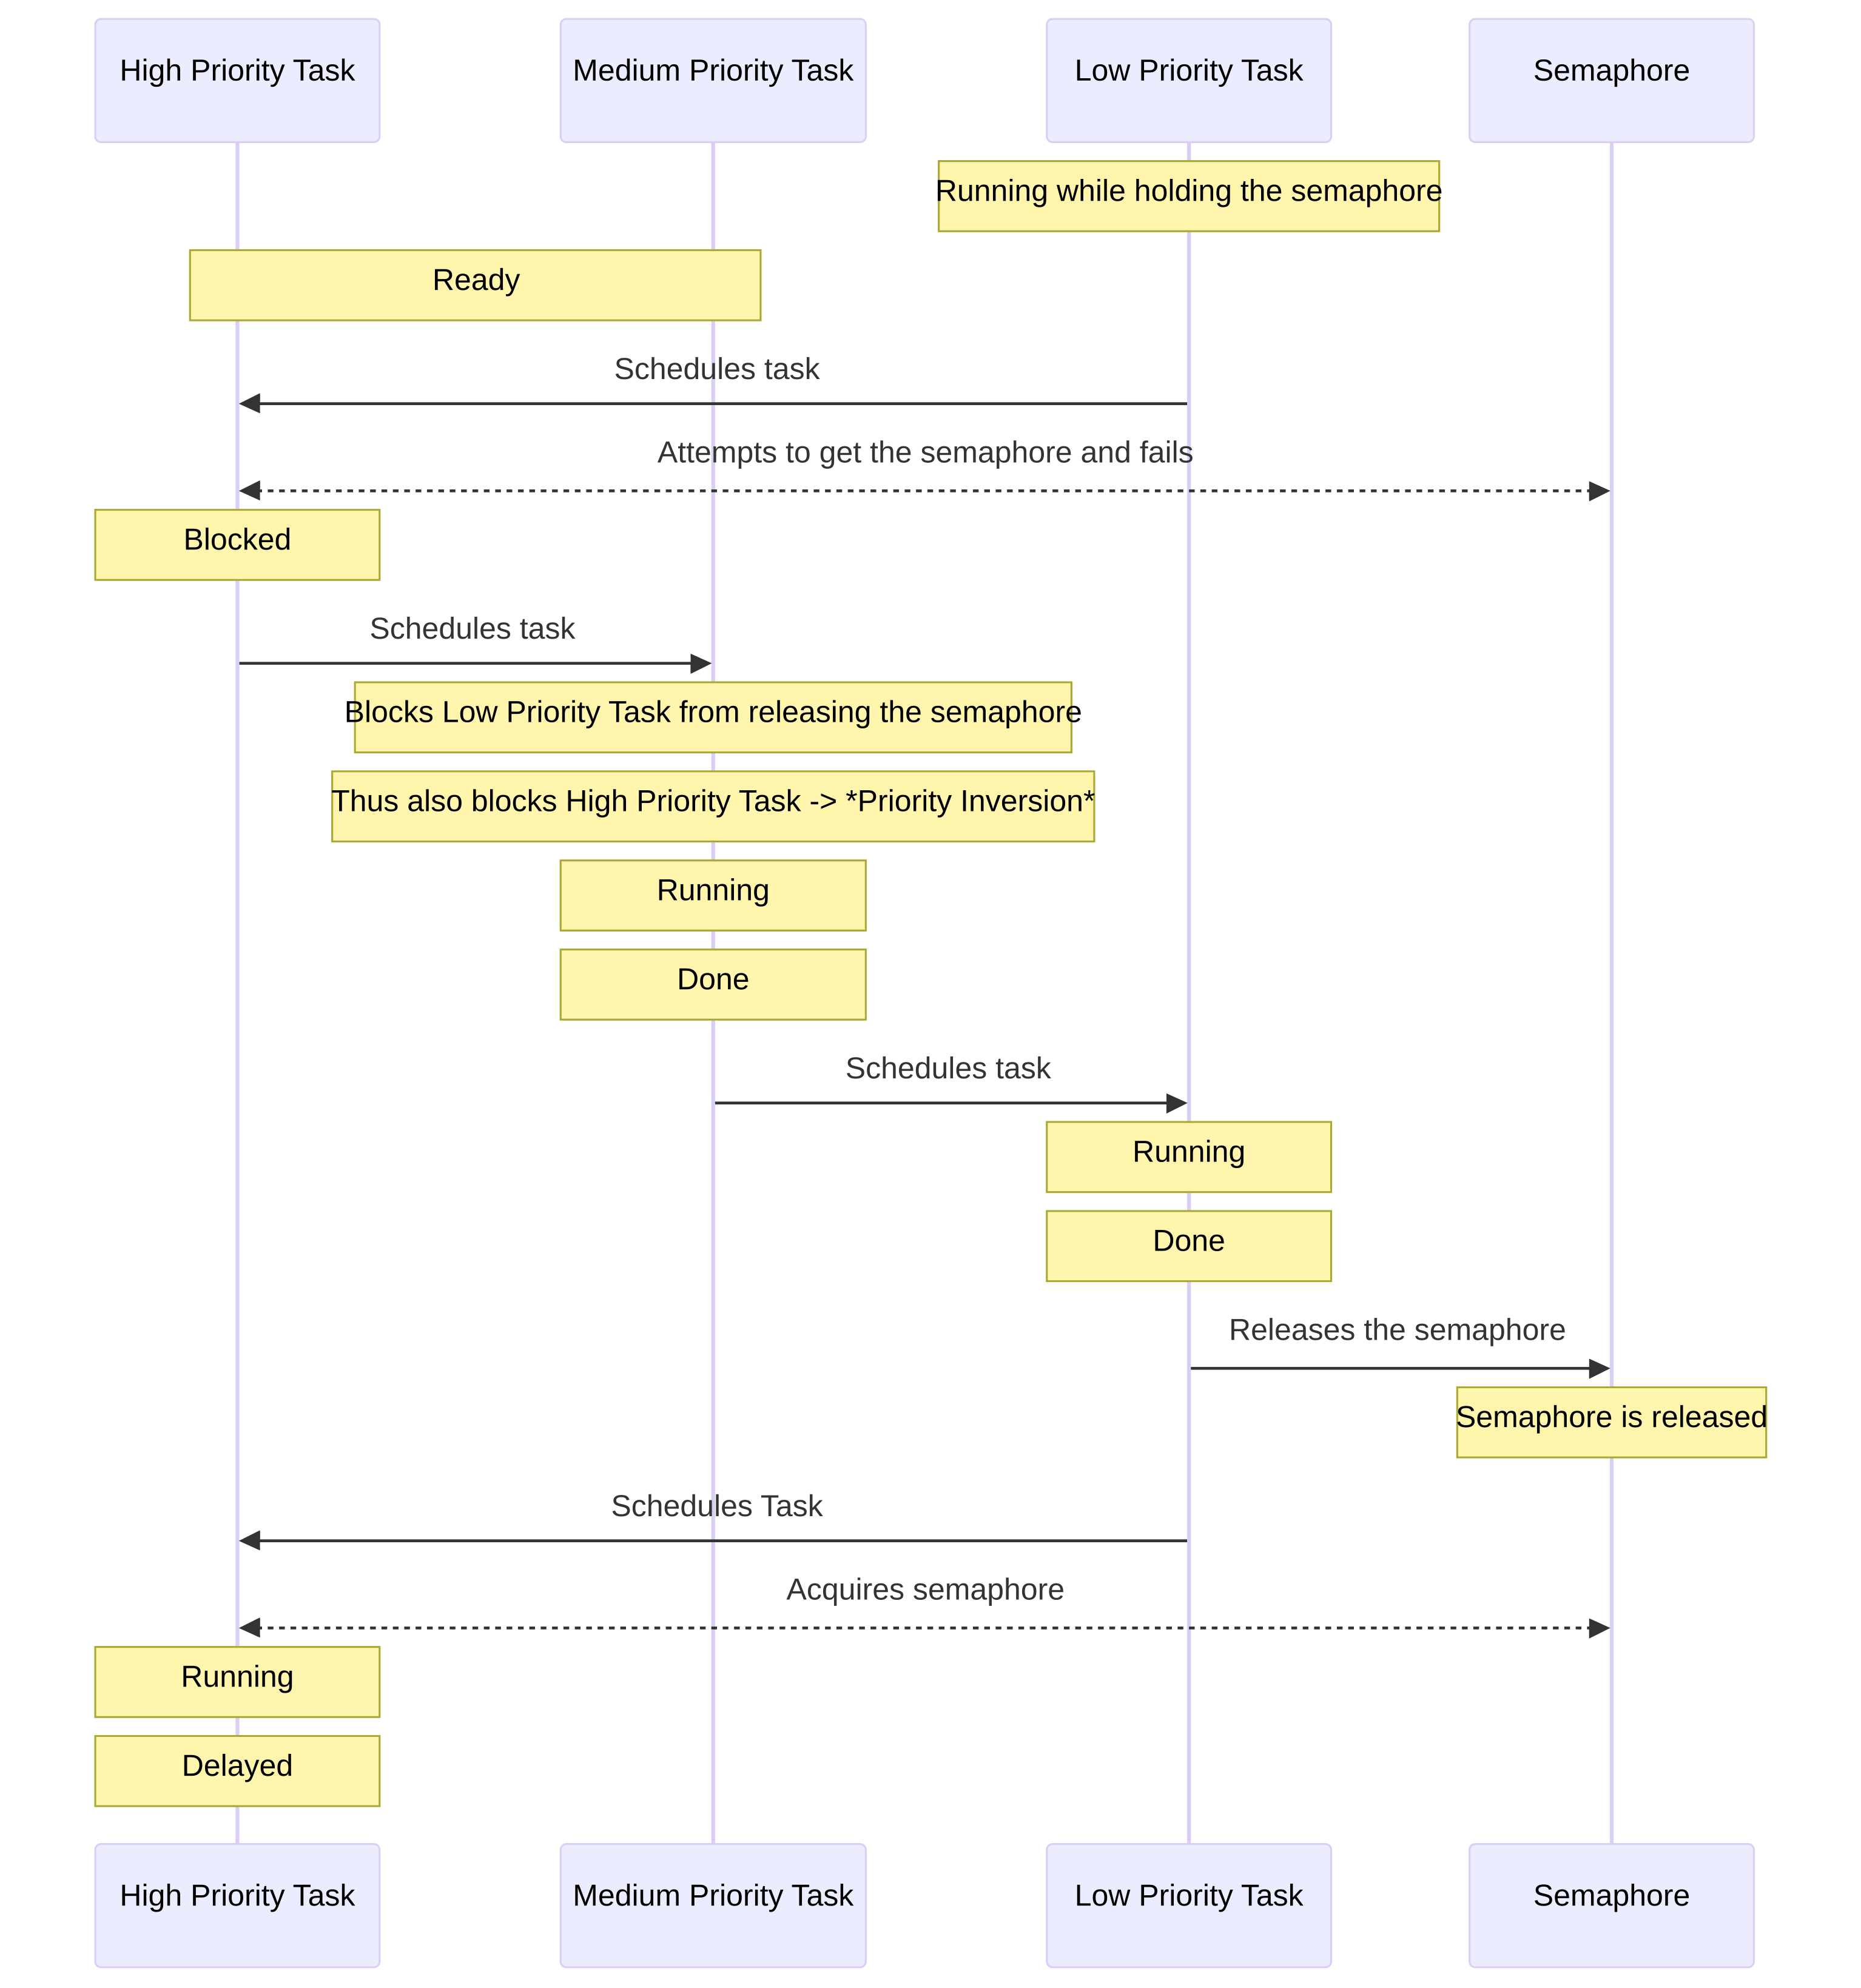
\includegraphics[width=1\textwidth]{assets/prio_inversion}
    \caption{Prioritätsinversion}
\end{figure}

\begin{figure}[H]
    \centering
    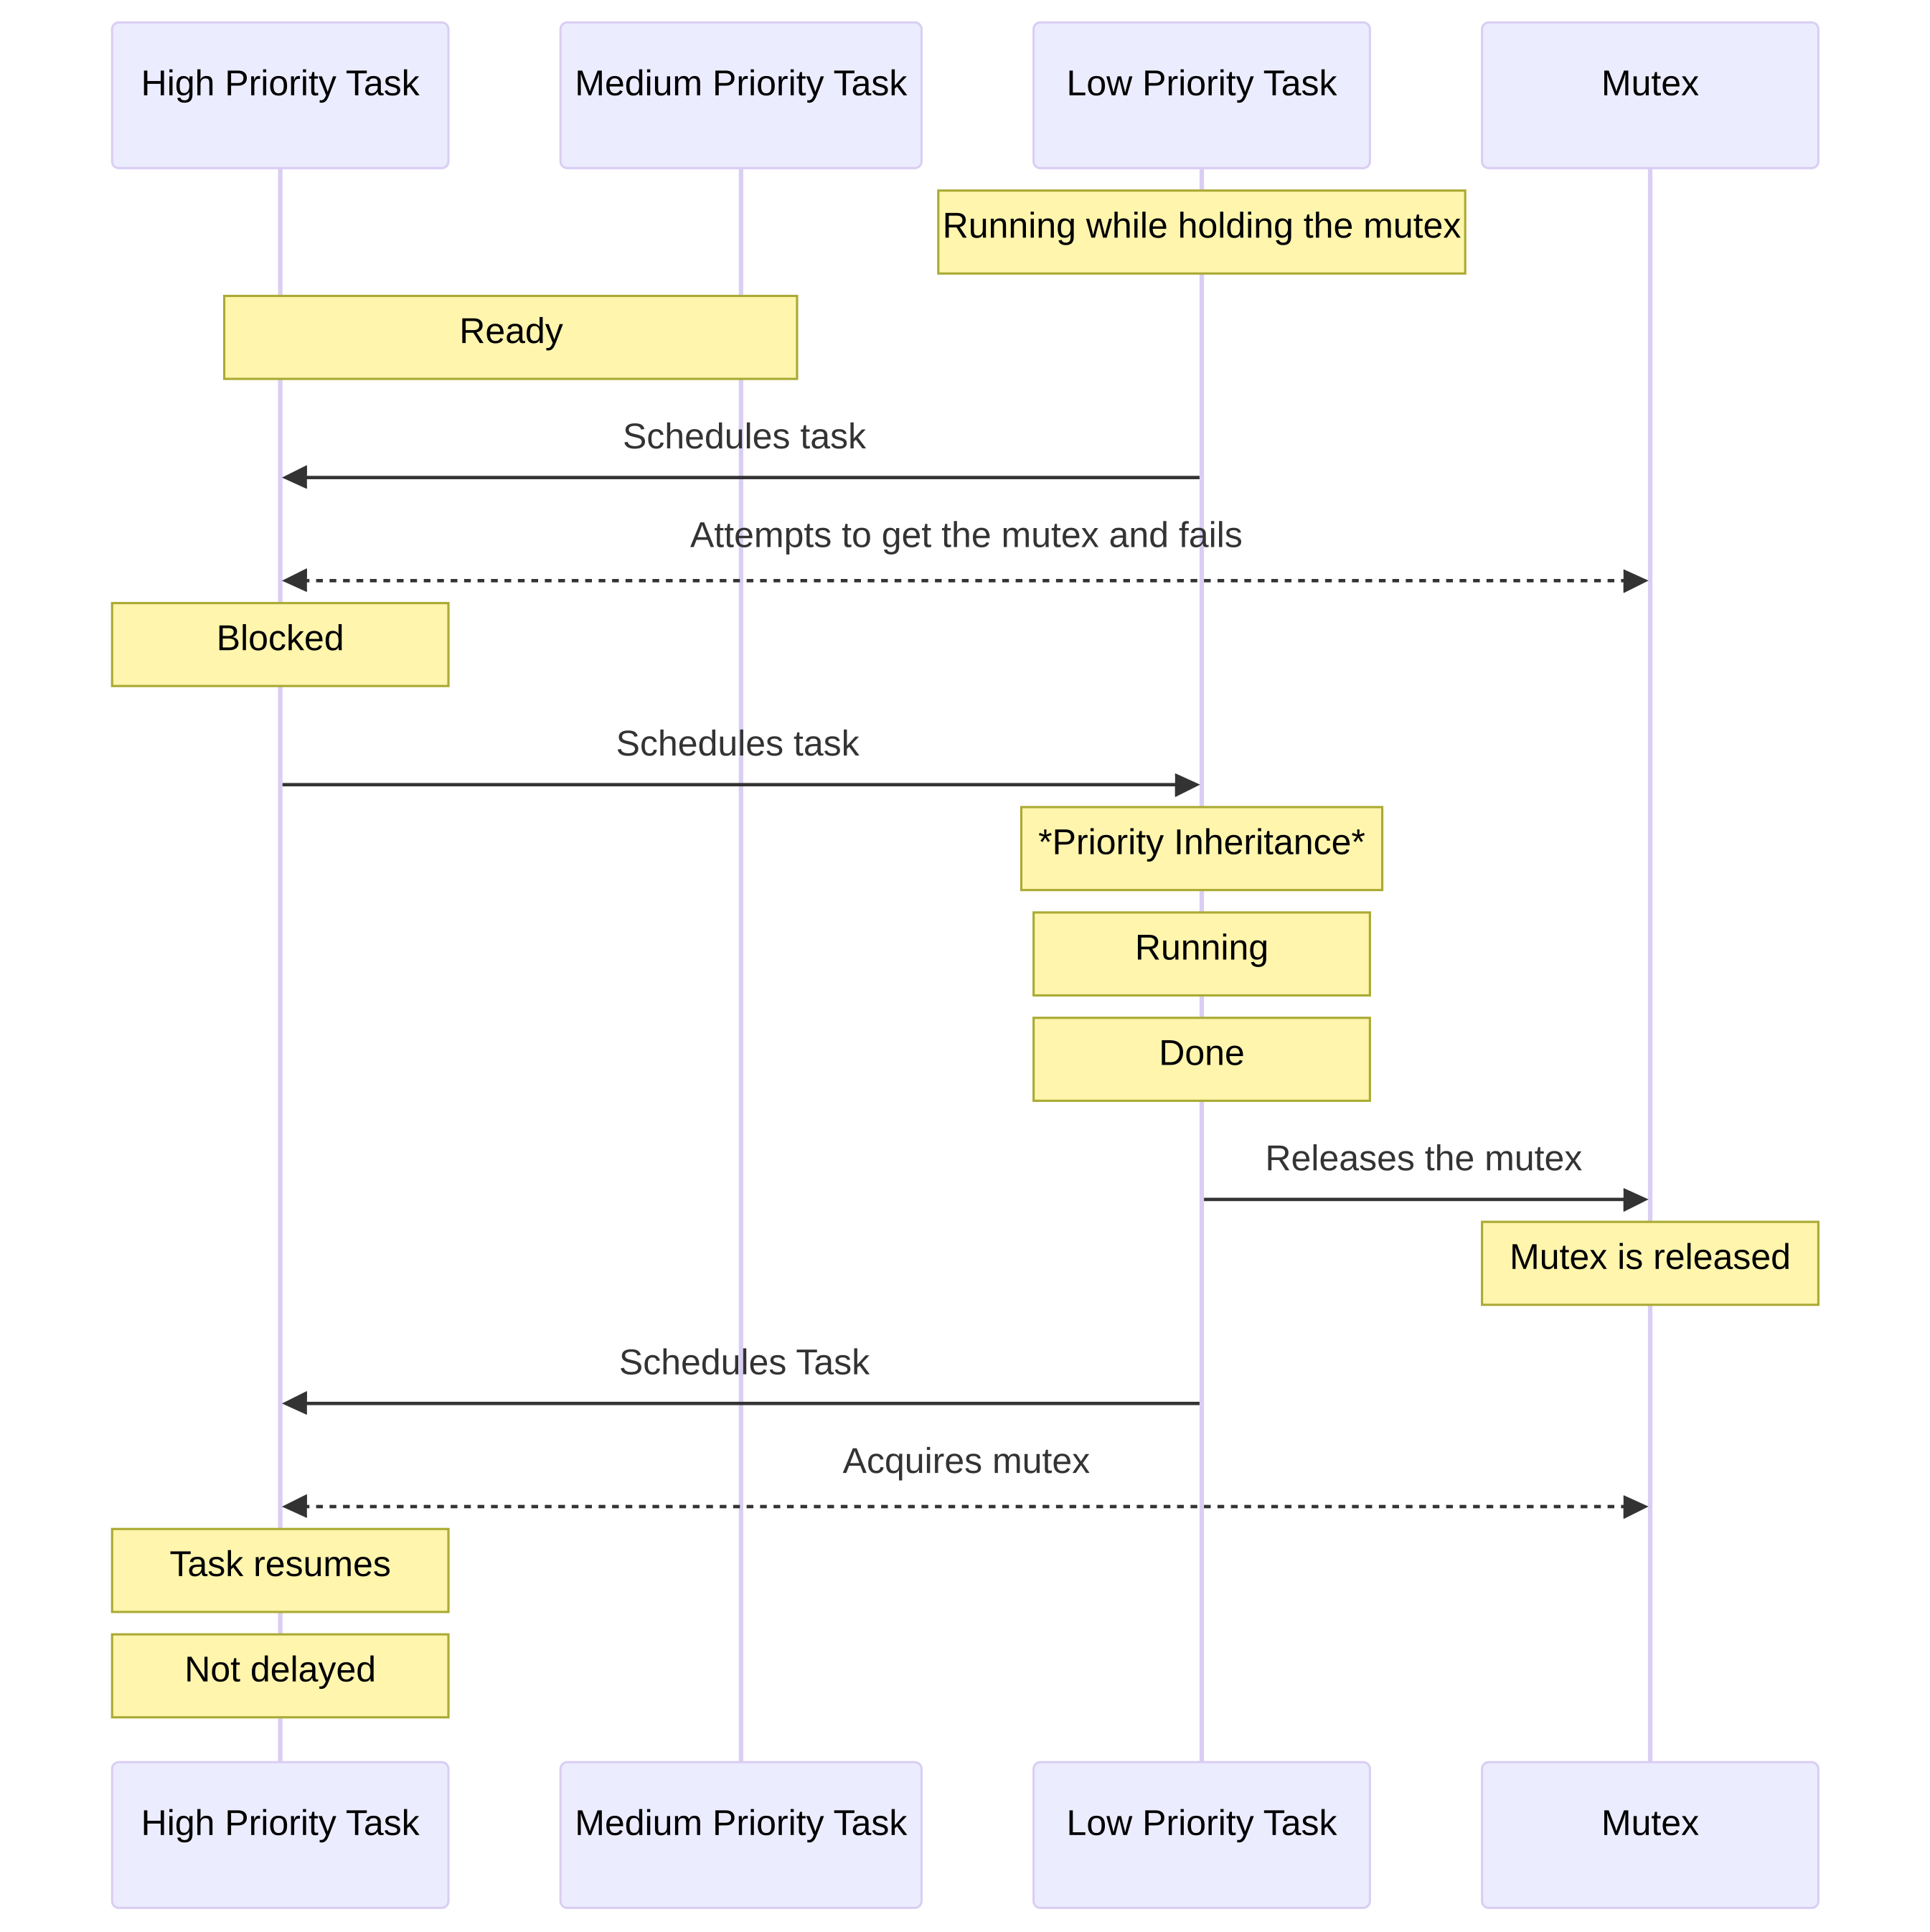
\includegraphics[width=1\textwidth]{assets/prio_inheritance}
    \caption{Prioritätsvererbung}
\end{figure}

\paragraph{Direct-Task-Notifications} \label{sec:direct_task_notification}

Direct-Task-Notifications sind ein effizienterer und ressourcenschonenderer
Mechanismus zur Inter-Task-Synchronisation: Insbesondere soll das Entblocken
mittels Direct-Task-Notifications bis zu $45\,\%$ schneller sein und weniger RAM
benötigen \cite{freertos_task_notifications_usage}. Im Gegensatz zu Semaphoren,
die als zusätzliche separate Objekte fungieren, koordinieren die Tasks direkt
miteinander über einen internen Zähler \cite{freertos_tasks_c_308}. Analog zur
Verwendung von Semaphoren wird mittels Funktionen wie
\mintinline{c}|xTaskNotifyGive()| dieser Zähler
inkrementiert~\cite{freertos_tasks_c_4990}, während
\mintinline{c}|ulTaskNotifyTake()| ihn wieder
dekrementiert~\cite{freertos_tasks_c_4614}.

\paragraph{Trace Hooks} \label{sec:trace_hooks}

„Trace Hooks“ sind spezielle, von FreeRTOS bereitgestellte Makros. Sie
ermöglichen beispielsweise die Verfolgung bzw. Protokollierung von
Systemereignissen. Diese Makros werden direkt innerhalb von Interrupts beim
Scheduling aufgerufen und sollten stets vor der Einbindung von
\mintinline{text}|FreeRTOS.h| definiert werden \cite{freertos_rtos_trace_hooks}.

\subsection{Caches}

Caches sind schnelle Speicherkomponenten, die häufige Daten- und Befehlzugriffe
beschleunigen und den Energieverbrauch senken, wodurch jedoch die
Determinierbarkeit der Leistung verringert wird \cite{ka001150}. In modernen
Mikrocontrollern wie dem Cortex-M7 ist der L1-Cache (Level 1 Cache -- die
kleinste aber schnellste Cachekomponente) jeweils in einen Datencache (D-Cache)
sowie einen Instruktionscache (I-Cache) unterteilt \cite[S. 6]{an4667}. Im
Vergleich zum Flash-Speicher, bei dem Zugriffe mehrere Taktzyklen
erfordern~\cite{stm32_memory_sections}, ermöglichen L1-Caches
Zero-Wait-State-Zugriffe~\cite[S. 6]{an4667}: der Prozessor kann ohne
zusätzliche Wartezyklen auf Daten zugreifen.

Der L1-Cache kann nur mit der \ac{AXI}-Busschnittstelle genutzt werden~\cite[S.
4]{an4839}. Hierzu zählen unter anderem der Flash, der \ac{SRAM} sowie die
Peripheriebusse, die alle über den \ac{AHB}-Bus an die AXI angebunden sind
(\ref{fig:m7_sys_arch}).

\begin{figure}[htb]
    \centering
    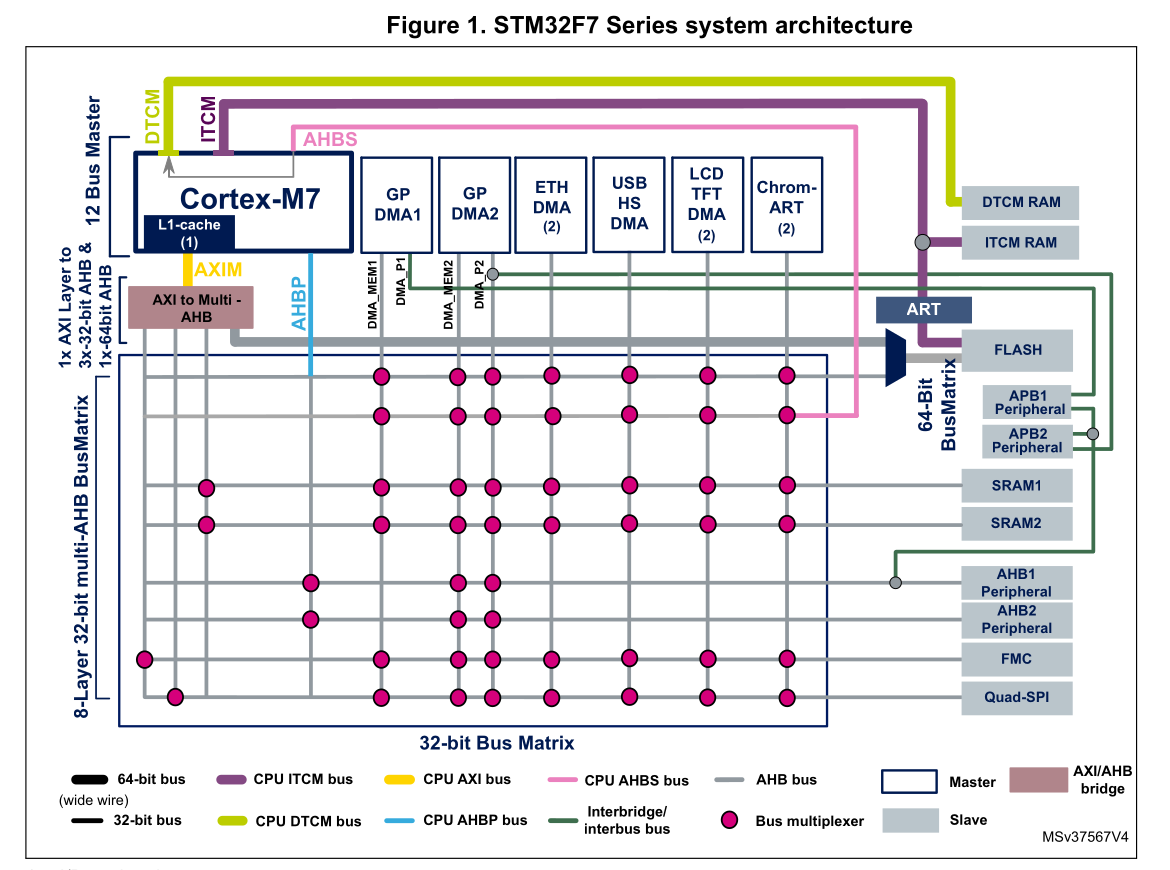
\includegraphics[width=1\textwidth]{assets/m7_system_arch}
    \caption{STM32F7 Systemarchitektur \cite[S. 9]{an4667}}
    \label{fig:m7_sys_arch}
\end{figure}

Aus der Matrix wird außerdem deutlich, dass für den Speicher zwischen SRAM und
\ac{TCM}-RAM unterschieden wird. Der TCM verfügt jeweils für Instruktionen und
Daten über einen dedizierten Kanal direkt zum Prozessor und ist \textit{nicht}
cachefähig, bietet aber als Besonderheit niedrigere und konsistente
Zugriffszeiten als SRAM. Dies macht sie besonders geeignet für zeitkritische
Routinen wie Interrupt-Handler oder kritische Echtzeitaufgaben.
(\cite{arm_den0042})

Im Rahmen dieser Bachelorarbeit wird der TCM nicht genutzt und daher nicht
weiter betrachtet.

Zusammenfassend lässt sich sagen, dass jeder normale Speicherbereich (kein
Shared-Memory, Device-Memory oder Strongly-Ordered-Memory) gecacht werden kann
\cite[S. 7]{an4667}, sofern er über den AXI-Bus zugänglich ist.

\begin{figure}[htb]
    \centering
    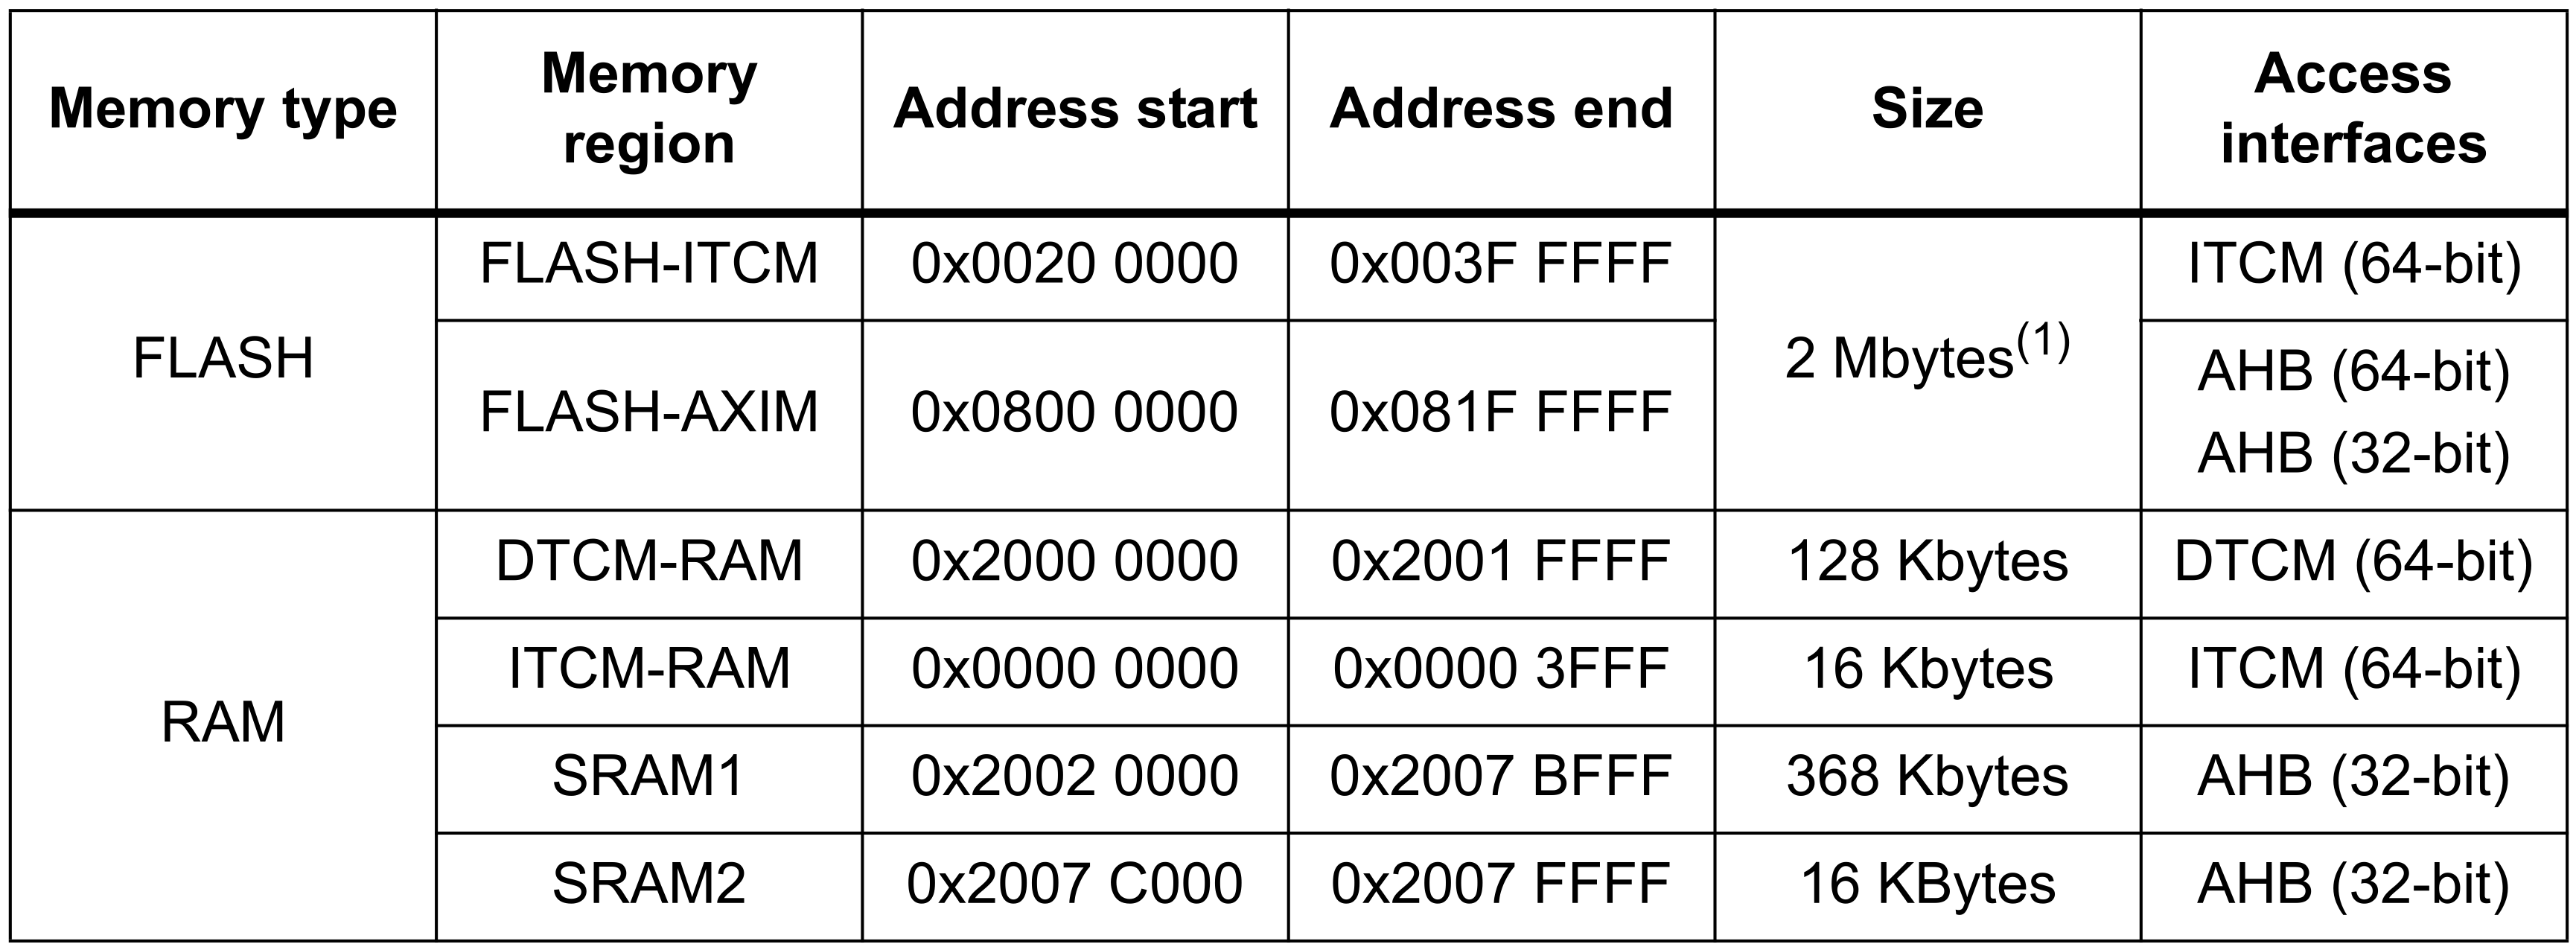
\includegraphics[width=1\textwidth]{assets/internal_mem_table}
    \caption{STM32F7 Speicheradressen \cite[S. 14]{an4667}}
    \label{fig:internal_mem_table}
\end{figure}

Aus der Tabelle \ref{fig:internal_mem_table} wird deutlich, dass der Flash ab
der Adresse $0x0800 0000$ über der AXI-Bus angesprochen wird . Diese Adresse ist
auch im Linker-Skript standardmäßig für den Flash festgelegt. Daher kann der
Instruktionscache über den AXI-Bus für den Flash genutzt werden, sofern der
Boot-Pin sowie die assoziierten \mintinline{text}|BOOT_ADDx|
Registerkonfigurationen korrekt eingestellt sind \cite[S. 28]{stm32_datasheet}
und die Firmware an die Standardadresse geflasht und gestartet wird.

\begin{code}
\begin{minted}{c}
MEMORY
{
RAM (xrw)      : ORIGIN = 0x20000000, LENGTH = 512K
FLASH (rx)      : ORIGIN = 0x8000000, LENGTH = 2048K
}
\end{minted}
    \captionof{listing}{Definition Speicherbereich im Linker-Script für STM32F7}
\end{code}

Um Caches zu nutzen, bietet die \ac{HAL} von STM32 dedizierte Funktionen als API
an \cite[S. 4]{an4839}:

\begin{code}
\begin{minted}{c}
void SCB_EnableICache(void)
void SCB_EnableDCache(void)
void SCB_DisableICache(void)
void SCB_DisableDCache(void)
void SCB_InvalidateICache(void)
void SCB_InvalidateDCache(void)
void SCB_CleanDCache(void)
void SCB_CleanInvalidateDCache(void)
\end{minted}
    \captionof{listing}{Cache-Funktionen}
\end{code}

\paragraph{Cache-Leerung} \label{sec:cache_clean}

Bei einer Cache-Leerung (cache clean) werden die modifizierten Cache-Zeilen, die
vom Prozessor während der Programmausführung aktualisiert wurden, zurück in den
Hauptspeicher geschrieben. Dieser Vorgang wird gelegentlich auch als „flush”
bezeichnet.

\paragraph{Cache-Invalidierung} \label{sec:cache_invalidate}

Eine Cache-Invalidierung markiert hingegen den Cache als ungültig, so dass bei
dem nachfolgenden Zugriff auf die assoziierten Daten diese zwingend erneut aus
dem Hauptspeicher geladen und der Cache entsprechend aktualisiert werden.

\subsubsection{Cache-Kohärenz} \label{sec:cache_coherency}

Bei der Nutzung von Caches kann für Speicherbereiche, die mit dem DMA-Controller
geteilt werden, ein Cache-Kohärenzproblem (cache coherency) auftreten, da der
Prozessor in diesem Fall nicht mehr der einzige Master ist, der auf diese
Speicherbereiche zugreift.

Damit der DMA-Controller stets auf korrekte Daten zugreifen kann, ist eine
manuelle Cache-Leerung (\ref{sec:cache_clean}) \textit{nach} jedem
Schreibvorgang von Seiten der CPU erforderlich \cite[S. 6]{an4839}. Ohne diesen
Schritt würden die Änderungen nicht umgehend im Speicher widergespiegelt, und
der DMA-Controller würde in der Zwischenzeit auf die veralteten und somit
ungültigen Daten zugreifen.

Bei Daten, die aus einem Speicherbereich gelesen werden, der auch vom
DMA-Controller modifiziert werden kann, ist \textit{vor} jedem Lesevorgang eine
Cache-Invalidierung (\ref{sec:cache_invalidate}) notwendig
\cite{embeddedexpert_cache}. Da der DMA-Controller asynchron und unabhängig von
der CPU schreiben kann, sind gecachten Daten immer potenziell veraltet, und
müssen stets manuell aktualisiert werden.

\subsection{Data Watchpoint and Trace Unit} \label{sec:dwt}

Für die Echtzeitfähigkeitsanalyse der Steuerungssoftware wird eine Methode
benötigt, die Code- bzw. Ausführungsabschnitte flexibel messen kann. Da es sich
dabei um eine mehrfädige Anwendung handelt, muss gewährleistet sein, dass die
Messungen trotz präemptives Scheduling, auftretender Interrupts sowie Software-
und Hardwareoptimierungen threadsicher und präzise durchgeführt werden. Die
endgültige Lösung muss garantieren, dass dabei keine Race Conditions entstehen
und auch die Zeiterfassung selbst keinen nennenswerten Overhead verursacht.

Daher bietet sich die \ac{DWT} als geeigneter Ansatz zur Protokollierung von
Laufzeiten an. Die DWT ist eine in ARM-Prozessoren eingebaute Debugging-Einheit,
die unter anderem ein funktionsreiches Profiling mittels verschiedener Zähler
unterstützen \cite{ARMv7_ref_man_dwt_profiling}. Ein für diese Arbeit zentraler
Baustein ist der Zyklenzähler \mintinline{c}|DWT_CYCCNT|, der bei jedem CPU-Takt
inkrementiert wird, solange sich der Prozessor nicht im Debug-Zustand befindet
\cite{ARMv7_ref_man_dwt_cycle}. Wie der Name des Zählers bereits vermuten lässt,
ermöglicht die DWT eine Laufzeit-Protokollierung mit \textit{zyklengenauer}
Präzision „unter normalen Betriebsbedingungen”
\cite{ARMv7_ref_man_dwt_profiling}.

\subsubsection*{Beispiel: Segger SystemView}

Ein Beispiel hierfür ist Segger SystemView, ein Echtzeitanalyse-Tool, das die
DWT nutzt, um Live-Code-Profiling auf eingebetteten Systemen durchzuführen
\cite{SEGGER_SystemView}.

Das Segger SystemView nutzt den DWT-Zyklenzähler, indem die Funktion \linebreak
\mintinline{c}|SEGGER_SYSVIEW_GET_TIMESTAMP()| für Cortex-M3/4/7-Prozessoren
einfach auf die hardkodierte Registeradresse des
Zyklenzählers~\cite{Arm_DWT_Programmers_Model} zugreift \cite[S.
65]{Segger_SystemView_manual}, anstatt die interne Funktion
\mintinline{c}|SEGGER_SYSVIEW_X_GetTimestamp()| aufzurufen.

\newpage

\section{Vorbereitung}

Die Vorbereitungsphase umfasst die Umstellung auf FreeRTOS und damit die
vollständige Ablösung von Micro-ROS. Der Datenaustausch wird intern über
FreeRTOS-Queues realisiert, während die Task-Synchronisation auf
Direct-Task-Notification anstatt von Semaphoren basiert. Zusätzlich wird die
Eingabe von Sollgeschwindigkeiten über UART mit CRC implementiert. Die
Aktivierung des Caches bildet den Abschluss dieser Vorbereitungen. Die Details
zu diesen Maßnahmen werden in den folgenden Abschnitten erläutert.

\subsection{Umstellung auf FreeRTOS}

\subsubsection{Geschwindigkeitsempfang über UART auf Mikrocontroller}

In der bisherigen Implementierung wurde der Geschwindigkeitssollwert vom
Host-System über ROS2 von dem Micro-ROS-Agent an den Client auf den MCU
übertragen. Um die Abhängigkeit von Micro-ROS komplett zu beseitigen, muss die
Übertragung und Interpretierung der Geschwindigkeitssollwerte manuell
implementiert werden.

Es wird zunächst ein einfacher Struct \mintinline{cpp}|Vel2d| definiert, um die
Geschwindigkeitswerte zu interpretieren, die vom Benutzer an den MCU gesendet
werden.

\begin{code}
\begin{minted}{cpp}
struct Vel2d {
  double x;
  double y;
  double omega;
};
\end{minted}
    \captionof{listing}{Definition der Struktur für die Sollgeschwindigkeit}
\end{code}

Darauf aufbauend wird eine weitere Struct \mintinline{cpp}|Vel2dFrame|
definiert, die als UART-Daten-Frame dient. Dieser enthält ein zusätzliches Feld
\mintinline{cpp}|crc| für die CRC-Überprüfung und eine Methode
\mintinline{cpp}|compare()|, die einen lokal kalkulierten CRC-Wert als Parameter
entgegennimmt, um diesen mit dem empfangenen zu vergleichen. Mit dem Attribut
\linebreak\mintinline{cpp}|__attribute__((packed))| wird verhindert, dass
zusätzliches Padding für die Speicherausrichtung dieses Typs eingefügt wird,
Damit die über UART empfangenen Bytes direkt als Objekt dieses Typs
interpretiert werden können.

\begin{code}
\begin{minted}{cpp}
struct Vel2dFrame {
  Vel2d vel;
  uint32_t crc;

  bool compare(uint32_t rhs) { return crc == rhs; }
} __attribute__((packed));

inline constexpr std::size_t VEL2D_FRAME_LEN = sizeof(Vel2dFrame);
\end{minted}
    \captionof{listing}{Definition der Data-Frame für die Sollgeschwindigkeit}
\end{code}

Für die Übertragung über UART kann die Setup-Funktion \linebreak
\mintinline{cpp}|HAL_UARTEx_ReceiveToIdle_IT()| aus der STM32-HAL-Bibliothek
verwendet werden, um die serialisierten Bytes eines Data-Frames zu empfangen.
Sie nimmt das UART-Handle, die Adresse eines Datenpuffers und dessen Größe
entgegen und empfängt die eingehenden Daten über Interrupts in diesen vorab
zugewiesenen Puffer.

Dies ist gepaart mit einer Interrupt-Callback
\mintinline{cpp}|HAL_UARTEx_RxEventCallback()|, die entweder ausgelöst wird,
wenn - wie der Name der UART-Setup-Funktion bereits andeutet - die UART-Leitung
feststellt, dass die Übertragung für eine bestimmte Zeit (abhängig von der
Baudrate) inaktiv war, oder wenn der Puffer für die Übertragung voll ist, was
darauf hinweist, dass der gesamte Inhalt des Puffers verarbeitet werden kann
\cite{HAL_UARTEx_ReceiveToIdle_IT}. Der zweite Parameter dieser
Interrupt-Callback gibt die Größe der in den Puffer geschriebenen Daten an
\cite{HAL_UARTEx_RxEventCallback}.

Mit diesem Setup kann die Software nun Bytes beispielsweise über UART direkt von
einem Linux-Host-Rechner empfangen, der mit dem MCU-Board verbunden ist.

\begin{code}
\begin{minted}{cpp}
// preallocated buffer with the exact size of a data frame
static uint8_t uart_rx_buf[VEL2D_FRAME_LEN];
volatile static uint16_t rx_len;

void HAL_UARTEx_RxEventCallback(UART_HandleTypeDef* huart, uint16_t size) {
  if (huart->Instance != huart3.Instance) return;

  rx_len = size;
  static BaseType_t xHigherPriorityTaskWoken;
  configASSERT(task_handle != NULL);
  vTaskNotifyGiveFromISR(task_handle, &xHigherPriorityTaskWoken);
  portYIELD_FROM_ISR(xHigherPriorityTaskWoken);

  // reset reception from UART
  HAL_UARTEx_ReceiveToIdle_IT(&huart3, uart_rx_buf, sizeof(uart_rx_buf));
}

// setup reception from UART in task init
HAL_UARTEx_ReceiveToIdle_IT(&huart3, uart_rx_buf, sizeof(uart_rx_buf));
\end{minted}
    \captionof{listing}{Nutzung STM32-HAL-API für den Datenempfang über UART via
    Interrupt}
\end{code}

Um die empfangenen Bytes zu parsen, ohne dies aber während der Ausführung der
Interrupt-Callback zu tun, wird ein eigenständiger FreeRTOS-Task erstellt.
Diesem Task wird von der Interrupt-Callback mittels
\mintinline{cpp}|vTaskNotifyGiveFromISR()|
signalisiert~\ref{sec:direct_task_notification} und die empfangenen Bytes werden
wieder in ein Data-Frame deserialisiert, um die Geschwindigkeit und die CRC zu
extrahieren.

Demnach kann dann eine CRC zur Kontrolle lokal aus den empfangenen
Geschwindigkeitswert berechnet werden und sie mit der empfangenen vergleichen.
Durch die Nutzung der dedizierten CRC-Peripherie ist die Berechnung
beispielsweise auf einem STM32-F37x-Gerät das 60-fache schneller, und verwendet
dabei nur 1,6\% der Taktzyklen im Vergleich zur Softwareberechnung \cite[S.
9]{AN4187}.

\begin{code}
\begin{minted}{cpp}
  while (true) {
    ulTaskNotifyTake(pdTRUE, portMAX_DELAY);

    len = rx_len;  // access atomic by default on ARM
    if (len != VEL2D_FRAME_LEN) {
      ULOG_ERROR("parsing velocity failed: insufficient bytes received");
      continue;
    }

    auto frame = *reinterpret_cast<const Vel2dFrame*>(uart_rx_buf);
    auto* vel_data = reinterpret_cast<uint8_t*>(&frame.vel);
    if (!frame.compare(HAL_CRC_Calculate(
            &hcrc, reinterpret_cast<uint32_t*>(vel_data), sizeof(frame.vel)))) {
      ULOG_ERROR("crc mismatch!");
      ++crc_err;
      continue;
    }

    frame.vel.x *= 1000;  // m to mm
    frame.vel.y *= 1000;  // m to mm

    xQueueSend(freertos::vel_sp_queue, &frame.vel, NO_BLOCK);
  }
\end{minted}
    \captionof{listing}{FreeRTOS-Task Dauerschleife}
\end{code}

\subsubsection{Geschwindigkeitsübertragung über UART auf Host}

Um den vom Benutzer festzulegenden Geschwindigkeitssollwert für den mobilen
Roboter zu übertragen, ist dem MCU-Board, auf dem die Steuerungssoftware läuft,
physisch per UART mit einem Linux-Host (einem Raspberry Pi 5) verbunden. Auf dem
Host wird das vorhandene ROS2-Paket \mintinline{text}|teleop_twist_keyboard|
verwendet, um Geschwindigkeitseingaben des Benutzers über die Tastatur zu
interpretieren. Um die Werten über UART zu senden, wird ein kleiner ROS2-Node
als Brücke erstellt, der den Micro-ROS-Agent ersetzt.

Dabei empfängt der Node über das ROS2-Framework die Geschwindigkeitssollwerte
und überträgt sie zusammen mit der im Konstruktur kalkulierten CRC an die
UART-Schnittstelle, die als abstrahierter serieller Port geöffnet ist.

\begin{code}
\begin{minted}{cpp}
class Vel2dBridge : public rclcpp::Node {
 public:
  Vel2dBridge() : Node{"vel2d_bridge"} {
    twist_sub_ = create_subscription<Twist>(
        "cmd_vel", 10, [this](Twist::UniquePtr twist) {
          auto frame =
              Vel2dFrame{{twist->linear.x, twist->linear.y, twist->angular.z}};

          if (!uart.send(frame.data())) {
            RCLCPP_ERROR(this->get_logger(), "write failed");
            return;
          }
          RCLCPP_INFO(this->get_logger(), "sending [%f, %f, %f], crc: %u",
                      frame.vel.x, frame.vel.y, frame.vel.omega, frame.crc);
        });
  }

 private:
  rclcpp::Subscription<Twist>::SharedPtr twist_sub_;
  SerialPort<VEL2D_FRAME_LEN> uart =
      SerialPort<VEL2D_FRAME_LEN>(DEFAULT_PORT, B115200);
};
\end{minted}
    \captionof{listing}{ROS2-Node Implementierung für
    Geschwindigkeitsübertragung}
\end{code}

Die CRC-Berechnung auf dem Host erfolgt mithilfe einer C++-Bibliothek von Daniel
Bahr \cite{CRCpp}. Der Algorithmus \mintinline{cpp}|CRC::CRC_32_MPEG2()|
entspricht demjenigen, der von der CRC-Peripherie des STM32-Boards verwendet
wird.

\begin{code}
\begin{minted}{cpp}
Vel2dFrame::Vel2dFrame(Vel2d vel)
    : vel{std::move(vel)},
      crc{CRC::Calculate(&vel, sizeof(vel), CRC::CRC_32_MPEG2())} {}
\end{minted}
    \captionof{listing}{CRC-Berechnung im Konstruktur}
\end{code}

Mithilfe dieser Implementierungen werden die Übertragung der
Geschwindigkeitssollwerte vom Host und deren Empfang auf dem MCU ermöglicht.
Dadurch, dass der Empfang detektiert, dass keine weiteren Bytes übertragen
werden, und ebenso durch die Überprüfung der CRC, werden unvollständige oder
fehlerhafte Bytes erkannt und verworfen, ohne den Programmablauf zu blockieren.

\subsubsection{Steuerungskomponenten als FreeRTOS-Task}

Analog zur Implementierung basierend auf Micro-ROS, bei der alle logischen
Komponenten als Single-Threaded-Executor abstrahiert werden, sind diese
Komponenten in FreeRTOS ebenfalls als eigenständige Tasks implementiert. Der
Fokus liegt hierbei darauf, den grundlegenden Datenaustausch in Form einer
Publisher-Subscriber-Architektur mittels Queues zu realisieren. Dadurch müssen
die Daten nicht mehr durch Semaphoren oder Mutexe geschützt werden, welche in
FreeRTOS auch nur mittels Queue-Objekte abstrahiert werden.

Zunächst wird ein eigenständiger Task zur Abfrage und Übertragung der
Encoderwerte erstellt, die von der Hardware bzw. der Hardwareabstraktion durch
Timer bereitgestellt werden, damit die anderen Tasks bei jeder Iteration auf
einheitliche Encoderwerte zugreifen können.

\begin{code}
\begin{minted}{cpp}
static void task_impl(void*) {
  constexpr TickType_t NO_BLOCK = 0;
  TickType_t xLastWakeTime = xTaskGetTickCount();
  const TickType_t xFrequency = pdMS_TO_TICKS(WHEEL_CTRL_PERIOD_MS.count());

  while (true) {
    auto enc_delta = FourWheelData(hal_encoder_delta_rad());

    xQueueSend(freertos::enc_delta_wheel_ctrl_queue, &enc_delta, NO_BLOCK);
    xQueueOverwrite(freertos::enc_delta_odom_queue, &enc_delta);

    vTaskDelayUntil(&xLastWakeTime, xFrequency);
  }
}
\end{minted}
    \captionof{listing}{FreeRTOS-Task für Encoderwertabfrage und -übertragung}
\end{code}


Der Empfänger-Task welchen mit \mintinline{cpp}|xQueueSend()| addressiert wird,
läuft mit einer höhreren Frequenz, sodass er die Daten immer sofort verarbeitet
und auf neue Daten wartet. Im Gegensatz dazu ist
\mintinline{cpp}|xQueueOverwrite()| eine spezielle Funktion, die ausschließlich
für Queues mit einer maximalen Kapazität von einem Objekt vorgesehen ist. Sie
überschreibt das vorhandene Objekt in der Queue, falls es existiert. In diesem
Kontext ist dies jedoch irrelevant, da der zugehörige Empfänger-Task, der mit
der gleichen Frequenz wie der Encoderwert-Task läuft, die Daten synchron
verarbeitet. Dennoch dient die Überschreibbarkeit als zusätzliche
Sicherheitsmaßnahme für den Fall, dass unerwartete Szenarien auftreten.

Darauf basierend kann die Kommunikation als Matrix wie folgt illustriert werden:

\begin{table}[h!]
\centering
\small
\setlength{\tabcolsep}{4pt} % Reduce column padding
\begin{tabular}{|c|c|c|c|}
\hline
    \diagbox{Sendertask}{Empfängertask} & \textbf{Odometrie} & \textbf{Drehzahlregelung} & \textbf{Posenregelung} \\ \hline
\textbf{Encoderwerte}               & $\rightarrow$             & $\rightarrow$       &               \\ \hline
\textbf{Geschwindigkeitssollwert}   &                           &                     & $\rightarrow$ \\ \hline
\textbf{Odometrie}                  & \cellcolor{gray!20}       &                     & $\rightarrow$ \\ \hline
\textbf{Drehzahlregelung}           &                           & \cellcolor{gray!20} & $\rightarrow$ \\ \hline
\end{tabular}
\caption{Kommunikationskanal-Matrix}
% \label{tab:kommunikationsmatrix}
\end{table}

Die Kanäle werden dementsprechend durch Queue-Objekte repräsentiert.

\begin{code}
\begin{minted}{cpp}
extern QueueHandle_t enc_delta_odom_queue;
extern QueueHandle_t enc_delta_wheel_ctrl_queue;
extern QueueHandle_t vel_sp_queue;
extern QueueHandle_t odom_queue;
extern QueueHandle_t vel_wheel_queue;
\end{minted}
    \captionof{listing}{Queue-Objekte in FreeRTOS}
\end{code}

Die grundlegende Implementierung der jeweiligen Steuerungstasks bleibt
größententeils von der Micro-ROS-Struktur erhalten. Die Initialisierung der
jeweiligen Steuerungstasks erfolgt in \mintinline{cpp}|freertos::init()|:

\begin{code}
\begin{minted}{cpp}
void init() {
  hal_init();
  queues_init();
  task_hal_fetch_init();
  task_vel_recv_init();
  task_pose_ctrl_init();
  task_wheel_ctrl_init();
  task_odom_init();
}
\end{minted}
    \captionof{listing}{Initialisierung von FreeRTOS-Tasks}
\end{code}

Eine üblicher Ansatz in einem FreeRTOS-System, um unter anderem sowohl den
Speicherverbrauch zu optimieren als auch die Programmdeterminiertheit zu
verbessern, besteht darin, die Erstellung der FreeRTOS-Objekte statisch
durchzuführen.

Um diese zu realisieren, wird im Makefile ein Macro
\mintinline{text}|-DFREERTOS_STATIC_INIT| definiert, das zur
Übersetzungszeit festlegt, ob die Objekte dynamisch innerhalb der FreeRTOS-API
oder statisch mit benutzerdefinierten Speicherorten zugewiesen werden sollen.

Für einen Task, der dynamisch allokiert wird, ist der Funktionsaufruf so einfach
wie der folgende:

\begin{code}
\begin{minted}{cpp}
xTaskCreate(task_impl, "hal_fetch", STACK_SIZE,
            NULL, osPriorityNormal, &task_handle);
\end{minted}
    \captionof{listing}{Dymanische Allokation eines FreeRTOS-Tasks}
\end{code}

Wenn ein Task statisch allokiert werden soll, muss der Benutzer manuell jeweils
einen Speicherpuffer für den Task-Stack und für den Task selbst deklarieren und
an die API übergeben.

\begin{code}
\begin{minted}{cpp}
static StackType_t taskStack[STACK_SIZE];
static StaticTask_t taskBuffer;
task_handle = xTaskCreateStatic(
                    task_impl, "hal_fetch", STACK_SIZE, NULL, osPriorityNormal,
                    taskStack, &taskBuffer);
\end{minted}
    \captionof{listing}{Dymanische Allokation eines FreeRTOS-Tasks}
\end{code}

Analog dazu muss der Benutzer für die statische Allokation einer Queue auch
jeweils einen Speicherpuffer mit der maximalen Kapazität für die Queue und für
die Queue selbst deklarieren:

\begin{code}
\begin{minted}{cpp}
 constexpr size_t QUEUE_SIZE = 10;
 static FourWheelData buf[QUEUE_SIZE];
 static StaticQueue_t static_queue;
 return xQueueCreateStatic(QUEUE_SIZE, sizeof(*buf),
                           reinterpret_cast<uint8_t*>(buf), &static_queue);
\end{minted}
    \captionof{listing}{Dymanische Allokation einer FreeRTOS-Queue}
\end{code}

Damit schließt der Abschnitt zur Umstellung auf FreeRTOS. Der Code für die
MCU-Software sowie für den ROS2-Node auf dem Host ist im
Repository~\cite{mecarover_freertos_profiling} verfügbar.

\newpage

\subsection{Aktivierung von Caches}

TODO

\newpage

\section{Implementierung zur Echtzeitanalyse}

Nachdem die Steuerungssoftware auf zwei verschiedenen Architekturen, nämlich
FreeRTOS und Micro-ROS, aufgebaut wurde, kann nun eine konkrete Implementierung
der Echtzeitanalyse basierend auf FreeRTOS erfolgen, um die Portabilität auf
Micro-ROS zu ermöglichen. Ziel der Analyse ist es, Informationen darüber zu
gewinnen, wie lange ein bestimmter Task oder eine bestimmte zeitkritische
Funktion benötigt. Die daraus resultierenden Daten müssen mit einer angemessenen
Genauigkeit erfasst werden, um sicherzustellen, dass die Echtzeitaspekte korrekt
widergespiegelt werden.

Aufgrund von Hardwarebeschränkungen sowie Einfachheit wurde UART als
Kommunikationsschnittstelle zur Übertragung der Echtzeitdaten vom
Mikrocontroller zum Host gewählt. Mit einer theoretischen Übertragungsrate von
bis zu 12,5 Mbit/s bietet UART ausreichende Bandbreite~\cite[S.
2]{stm32_datasheet}, um die Profiling-Daten zu übertragen, ohne Überlastung zu
verursachen.

Daraus ergibt sich als Erstes die Notwendigkeit, eine threadsichere \ac{MPSC}
Queue, oder besser gesagt eine multi-producer Senke, zu implementieren, welche
die Echtzeitdaten kontinuierlich konsumiert und sie über UART ausgibt. Die
FreeRTOS Stream- oder Messagebuffer sind für den Fall mit mehreren Producers
nicht geeignet~\cite{FreeRTOSStreamBuffer}.

\subsection{Threadsichere Senke}

Da FreeRTOS und dementsprechend auch Micro-ROS multithreaded sind und zur
Echtzeitanalyse von beliebiger Stelle beim Programmlauf Echtzeitdaten durch IO
übertragen werden, muss dabei die Thread-Sicherheit gewährleistet werden, damit
die zu übertragenden Daten nicht durch Race Conditions neu geordnet,
überschrieben oder zu unbrauchbaren Daten werden.

the basic idea is that data from multiple threads are pushed into the sink or
saved in a buffer, and are waiting to be consumed by a single consumer. because
storage is finite, the sink has to be able to know when to block further writing
data to the buffer thus overwriting the data yet to be consumed.

taking inspiration from a C++ conference talk from year
2024~\cite{CppCon2024LockFreeQueue}, where each position of the data buffer has
a unique sequence number, which, upon consumption, gets incremented atomically
by the total length of the data buffer, indicating that the data at this
position is ready to be overwritten at the next iteration by the writer, by
comparing it to the global write sequence number, can the multi-producer sink
with only one consumer only save a bool state whether the data at a specific
location is yet to be consumed or can be overwritten. % TODO


\subsection{Aktivierung der DWT}

Wie im vorherigen Abschnitt erläutert \ref{sec:dwt}, stellt die DWT einen
geeigneten Ansatz zur Generierung von Analysedaten dar. Sie ist standardmäßig
auf Cortex-M7-Prozessoren verfügbar und kann durch die folgenden
Konfigurationsschritte aktiviert werden:

\begin{code} \begin{minted}{cpp} void enable_dwt() { CoreDebug->DEMCR |=
CoreDebug_DEMCR_TRCENA_Msk; DWT->LAR = 0xC5ACCE55;  // software unlock
DWT->CYCCNT = 1; DWT->CTRL |= DWT_CTRL_CYCCNTENA_Msk; } \end{minted}
\captionof{listing}{Aktivierung der DWT \cite{StackOverflow_DWT_Activation}}
\end{code}

\newpage

\section{Evaluation}

\begin{figure}[h]
    \centering
    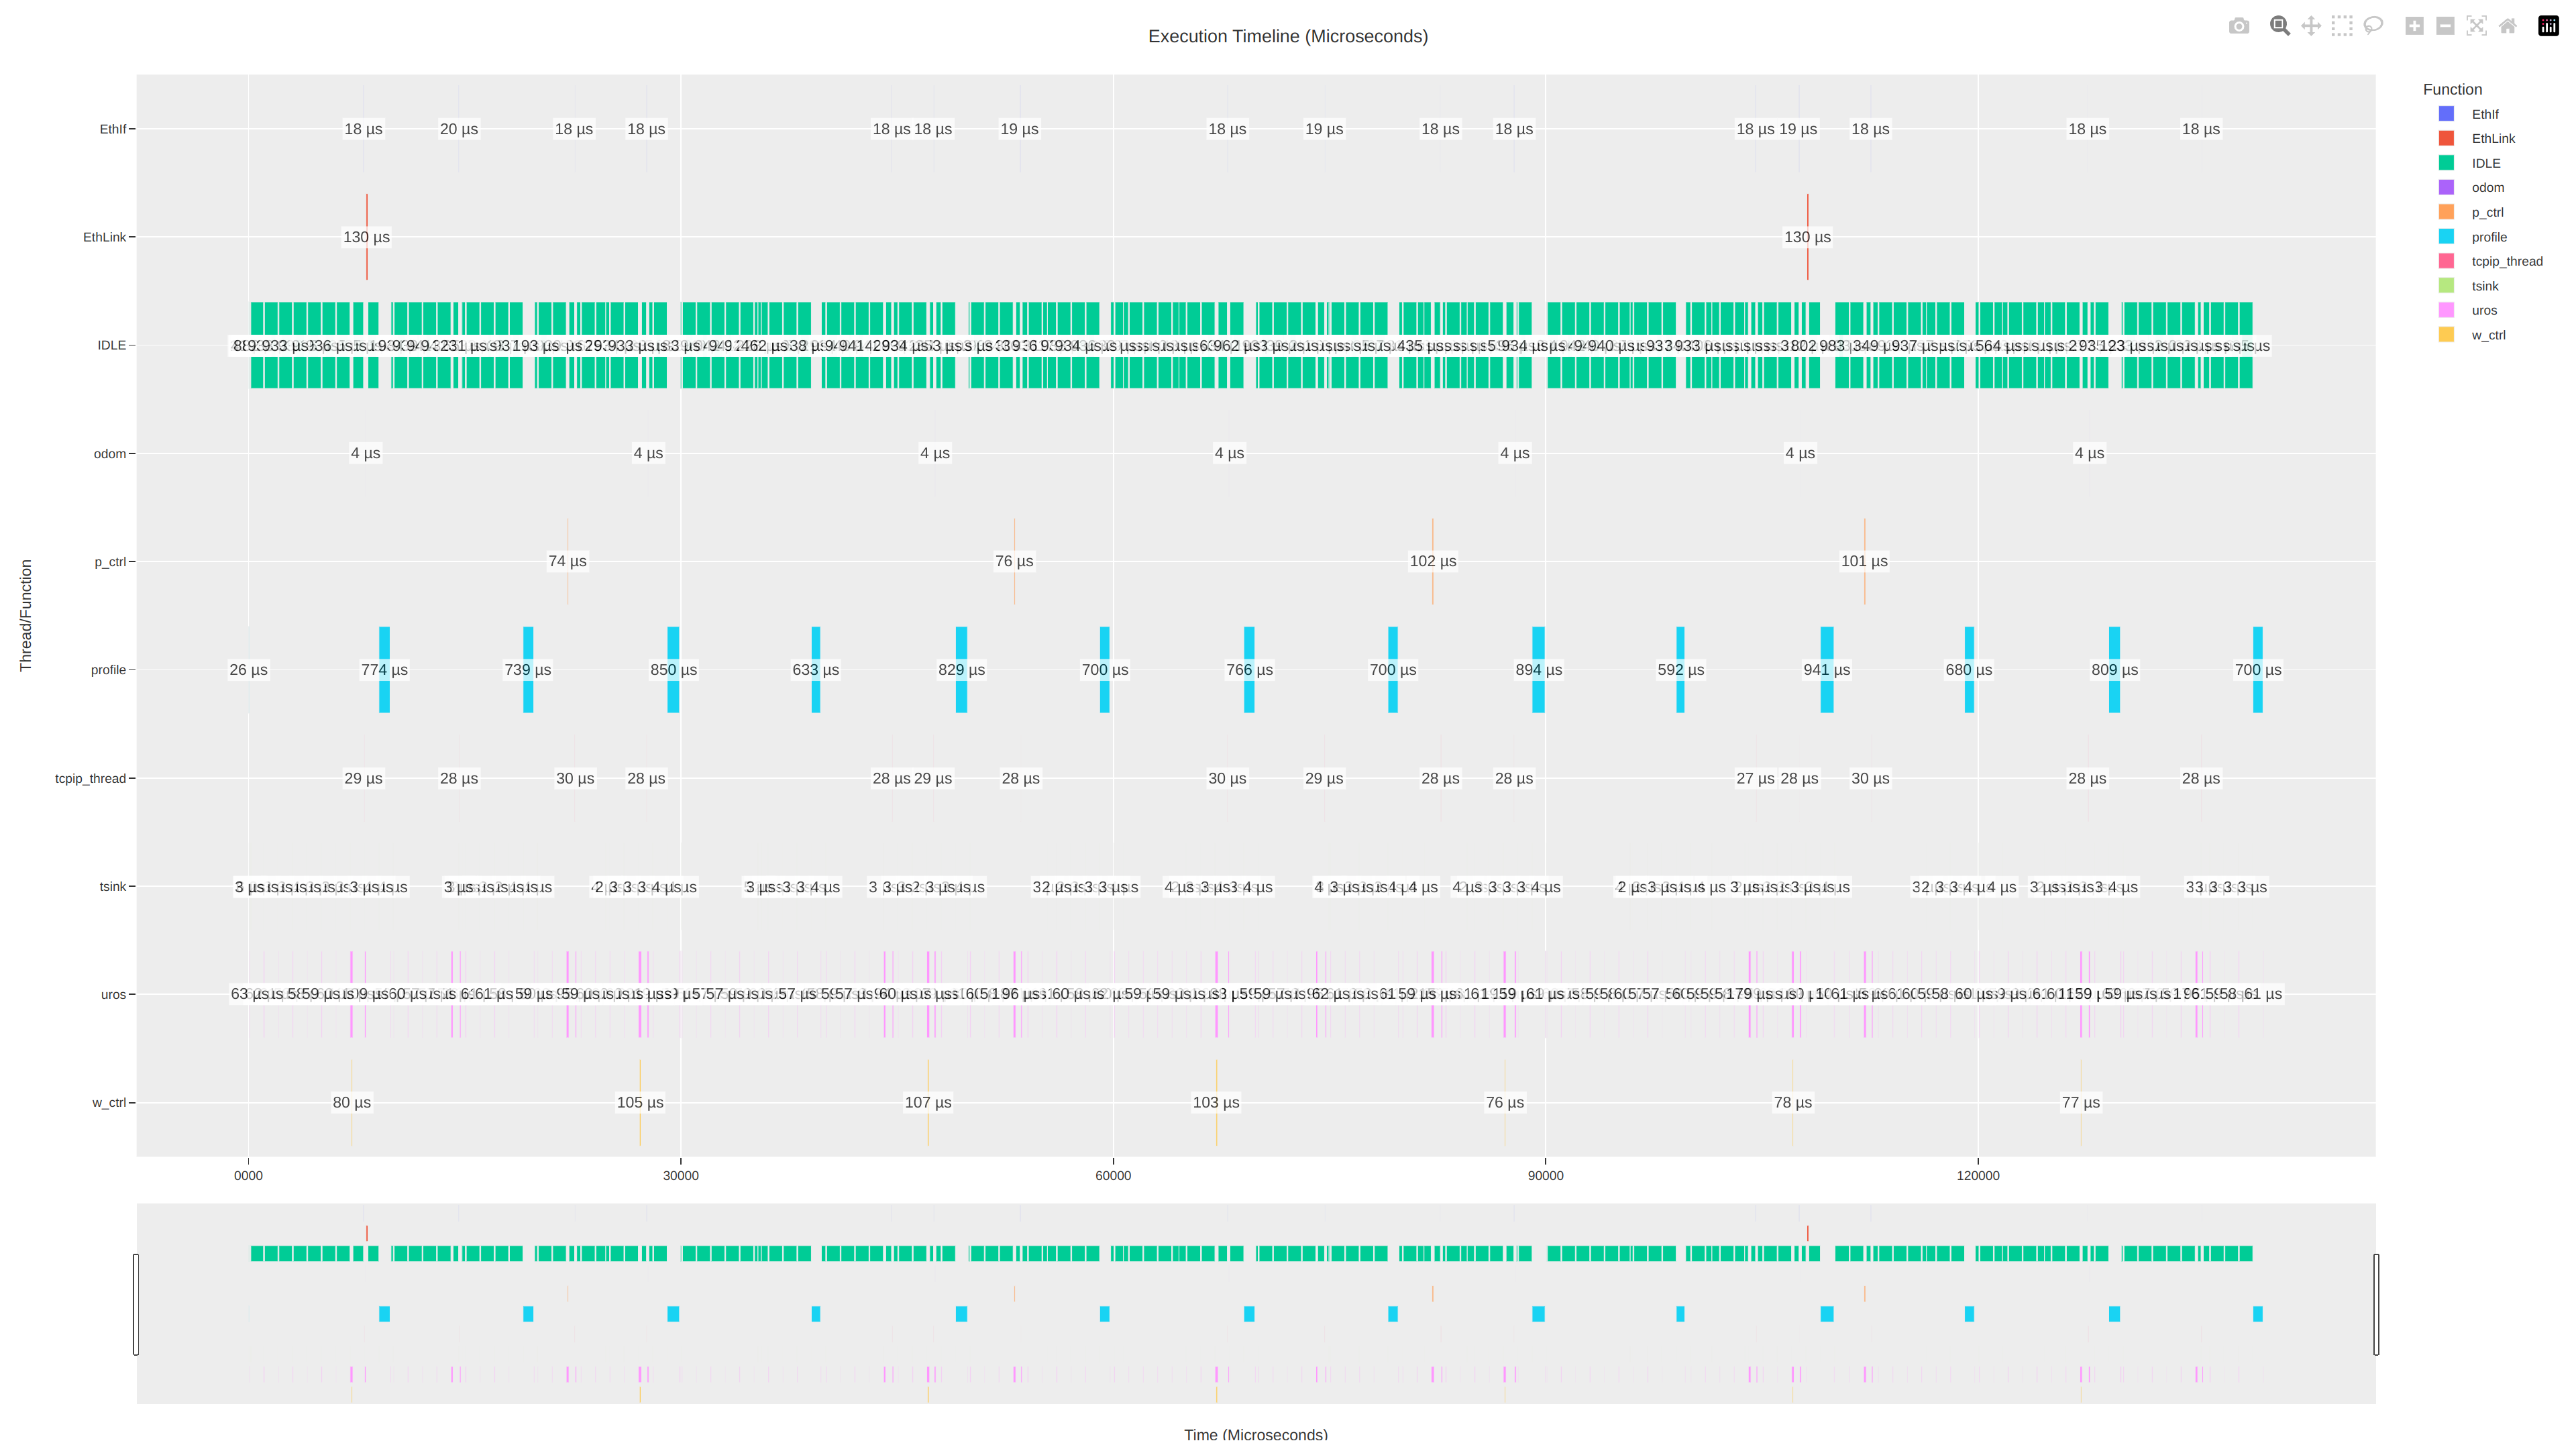
\includegraphics[width=1\textwidth]{assets/micro_ros_profiling}
    \caption{Visualisierung der Echtzeitanalyse unter Micro-ROS}
    % \label{fig:micro_ros_profiling}
\end{figure}

\begin{code}
\begin{minted}{cpp}
=======================================
free heap:          4688
ctx switches:       126810
Task            Time        %
profile         33450       2%
uros            106984      8%
IDLE            1179311     88%
EthLink         1695        <1%
tcpip_thread    4526        <1%
tsink           3762        <1%
Tmr Svc         0           <1%
EthIf           2730        <1%
---------------------------------------
Task        State   Prio    Stack   Num
uros            R     24     2548     3
profile         X     24     892      2
IDLE            R     0      108      4
tcpip_thread    B     24     180      6
tsink           B     32     475      1
EthLink         B     16     193      8
EthIf           B     48     17       7
Tmr Svc         B     2      223      5
=======================================
profiled for 18881864 us
\end{minted}
    \captionof{listing}{Zusammenfassung Echtzeitanalyse unter Micro-ROS}
\end{code}

\begin{figure}[h]
    \centering
    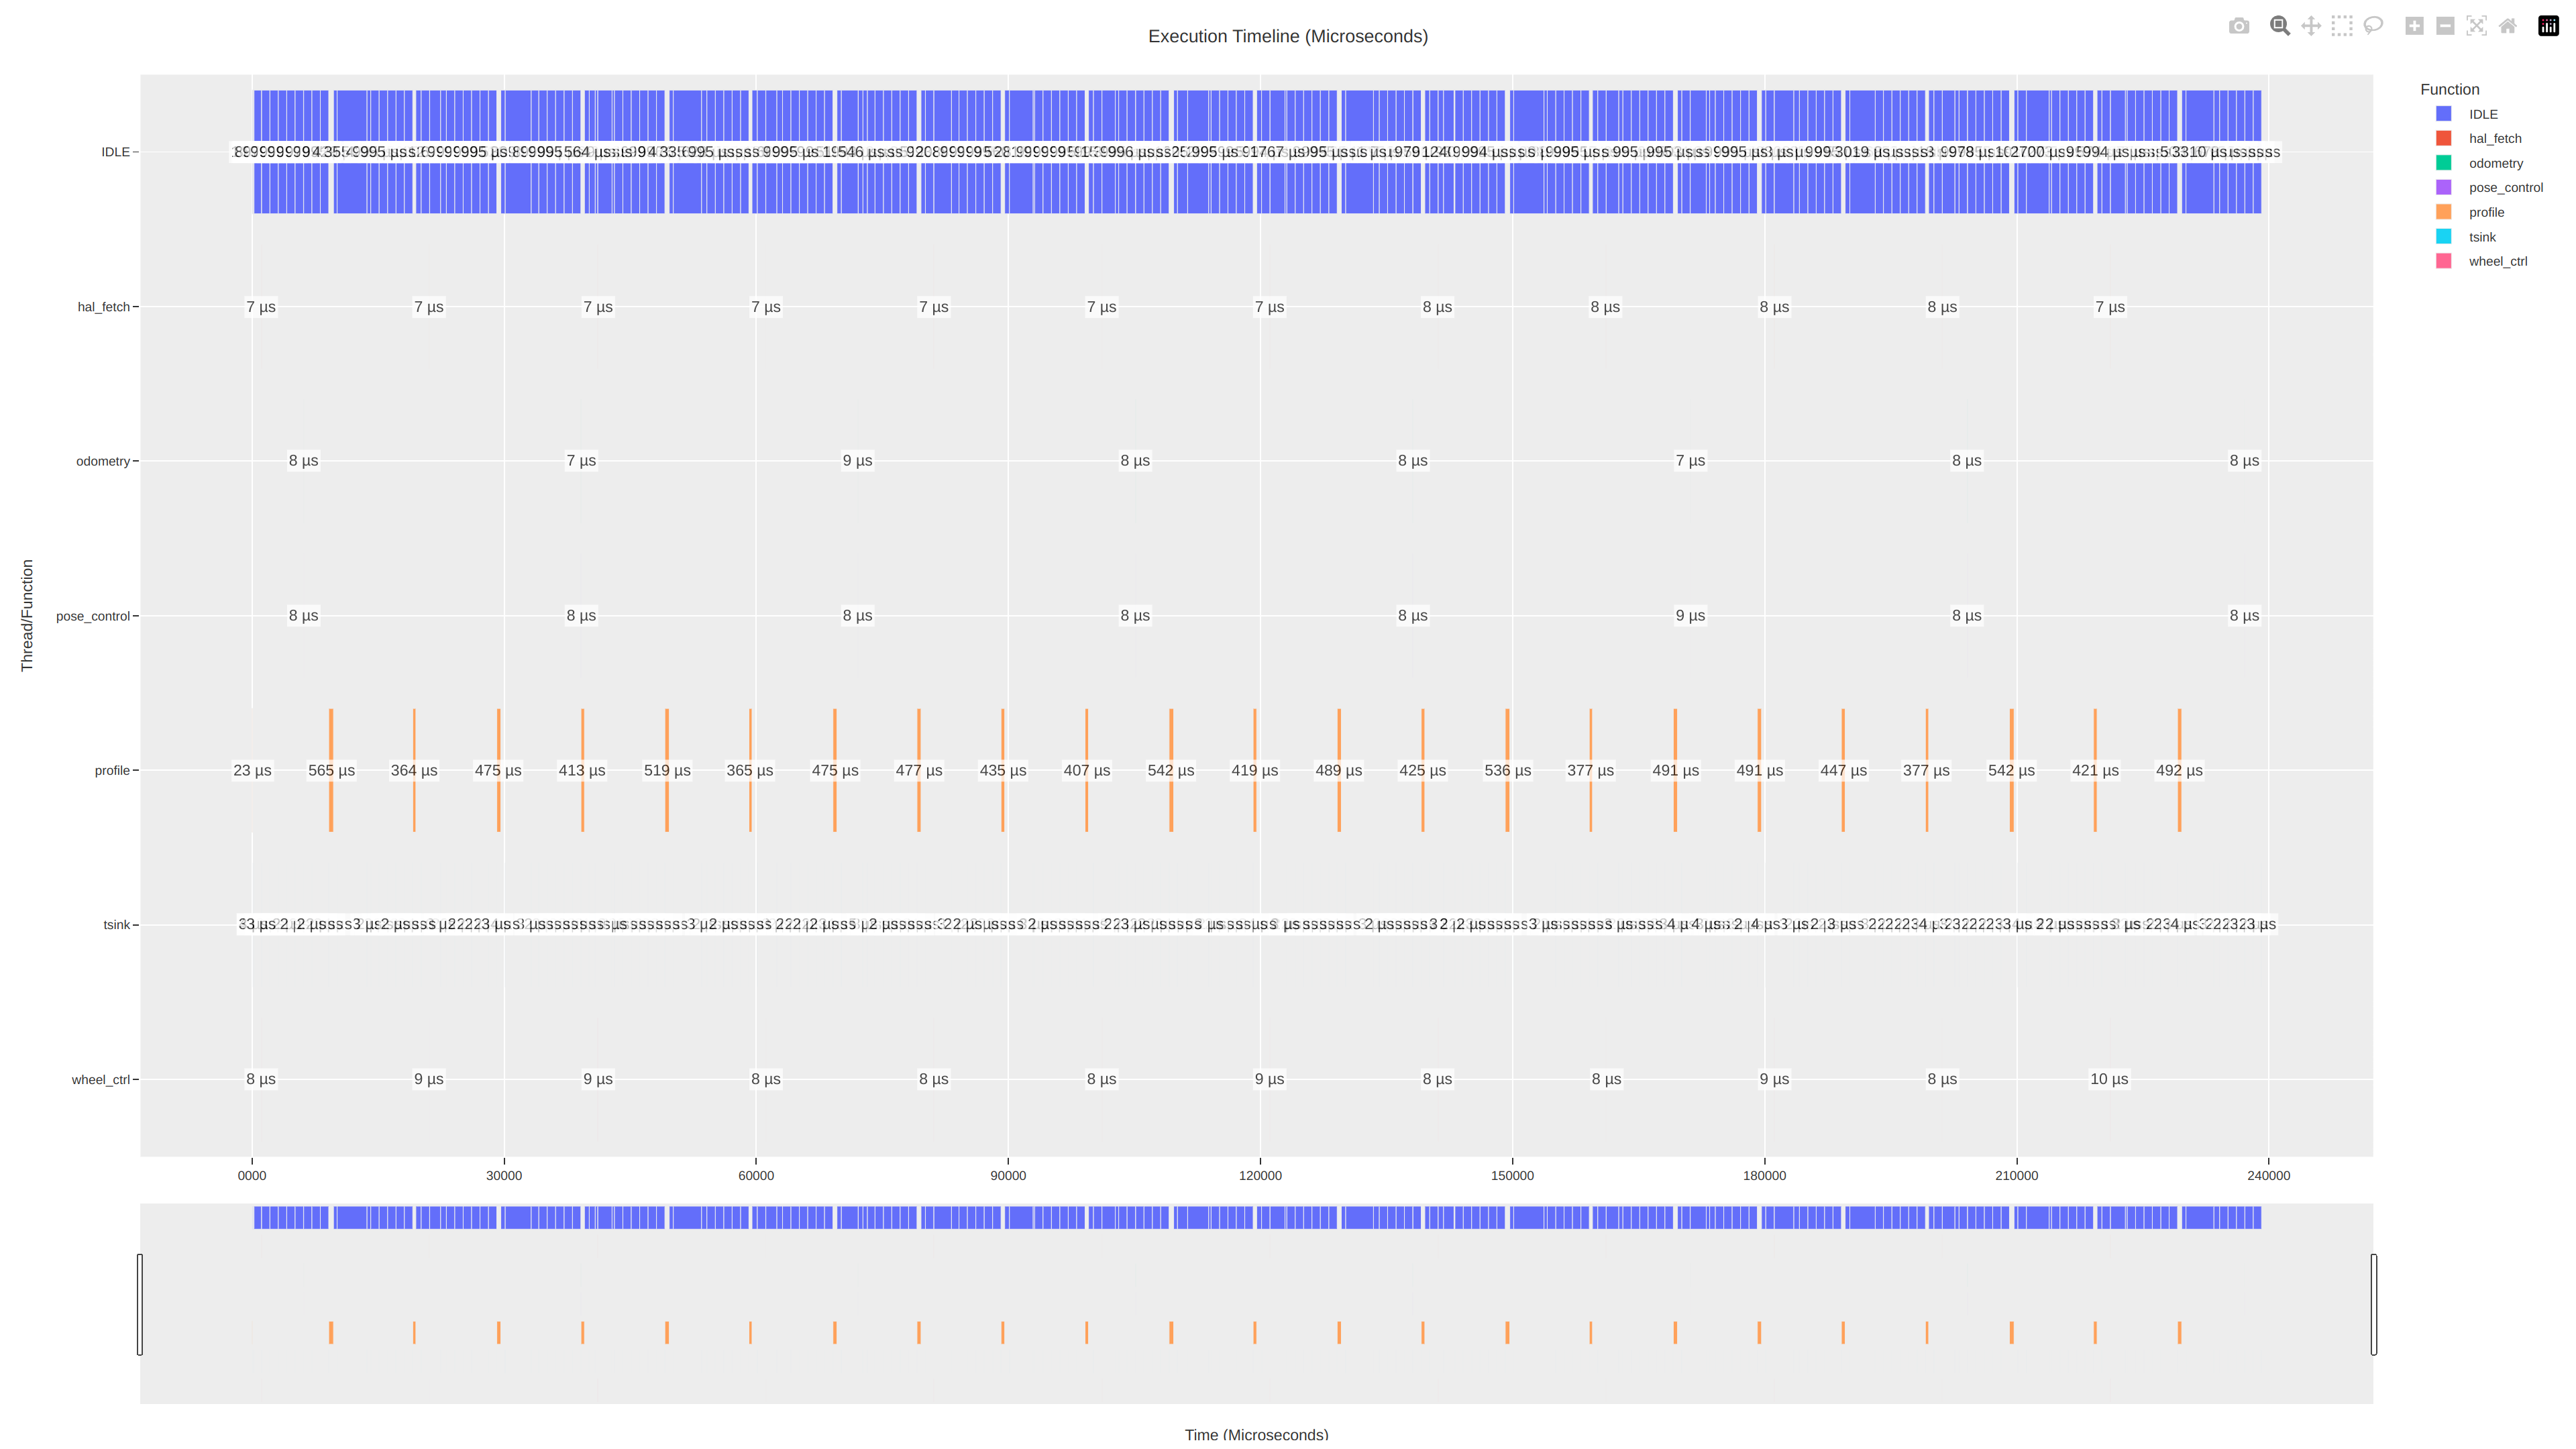
\includegraphics[width=1\textwidth]{assets/freertos_profiling}
    \caption{Visualisierung der Echtzeitanalyse unter FreeRTOS}
    % \label{fig:freertos_profiling}
\end{figure}

\begin{code}
\begin{minted}{cpp}
=======================================
free heap:          195696
ctx switches:       76148
Task            Time        %%
profile         9669        4%
IDLE            201086      95%
hal_fetch       81          <1%
wheel_ctrl      87          <1%
odometry        49          <1%
pose_control    51          <1%
tsink           615         <1%
Tmr Svc         0           <1%
recv_vel        0           <1%
---------------------------------------
Task        State   Prio    Stack   Num
profile         X      24     900     7
IDLE            R      0      108     8
wheel_ctrl      B      24     420     5
odometry        B      24     416     6
pose_control    B      24     410     4
tsink           B      32     483     1
hal_fetch       B      24     443     2
recv_vel        S      24     441     3
Tmr Svc         B      2      223     9
=======================================
profiled for 18779120 us
\end{minted}
    \captionof{listing}{Zusammenfassung Echtzeitanalyse unter Micro-ROS}
\end{code}

\begin{figure}[h]
    \centering
    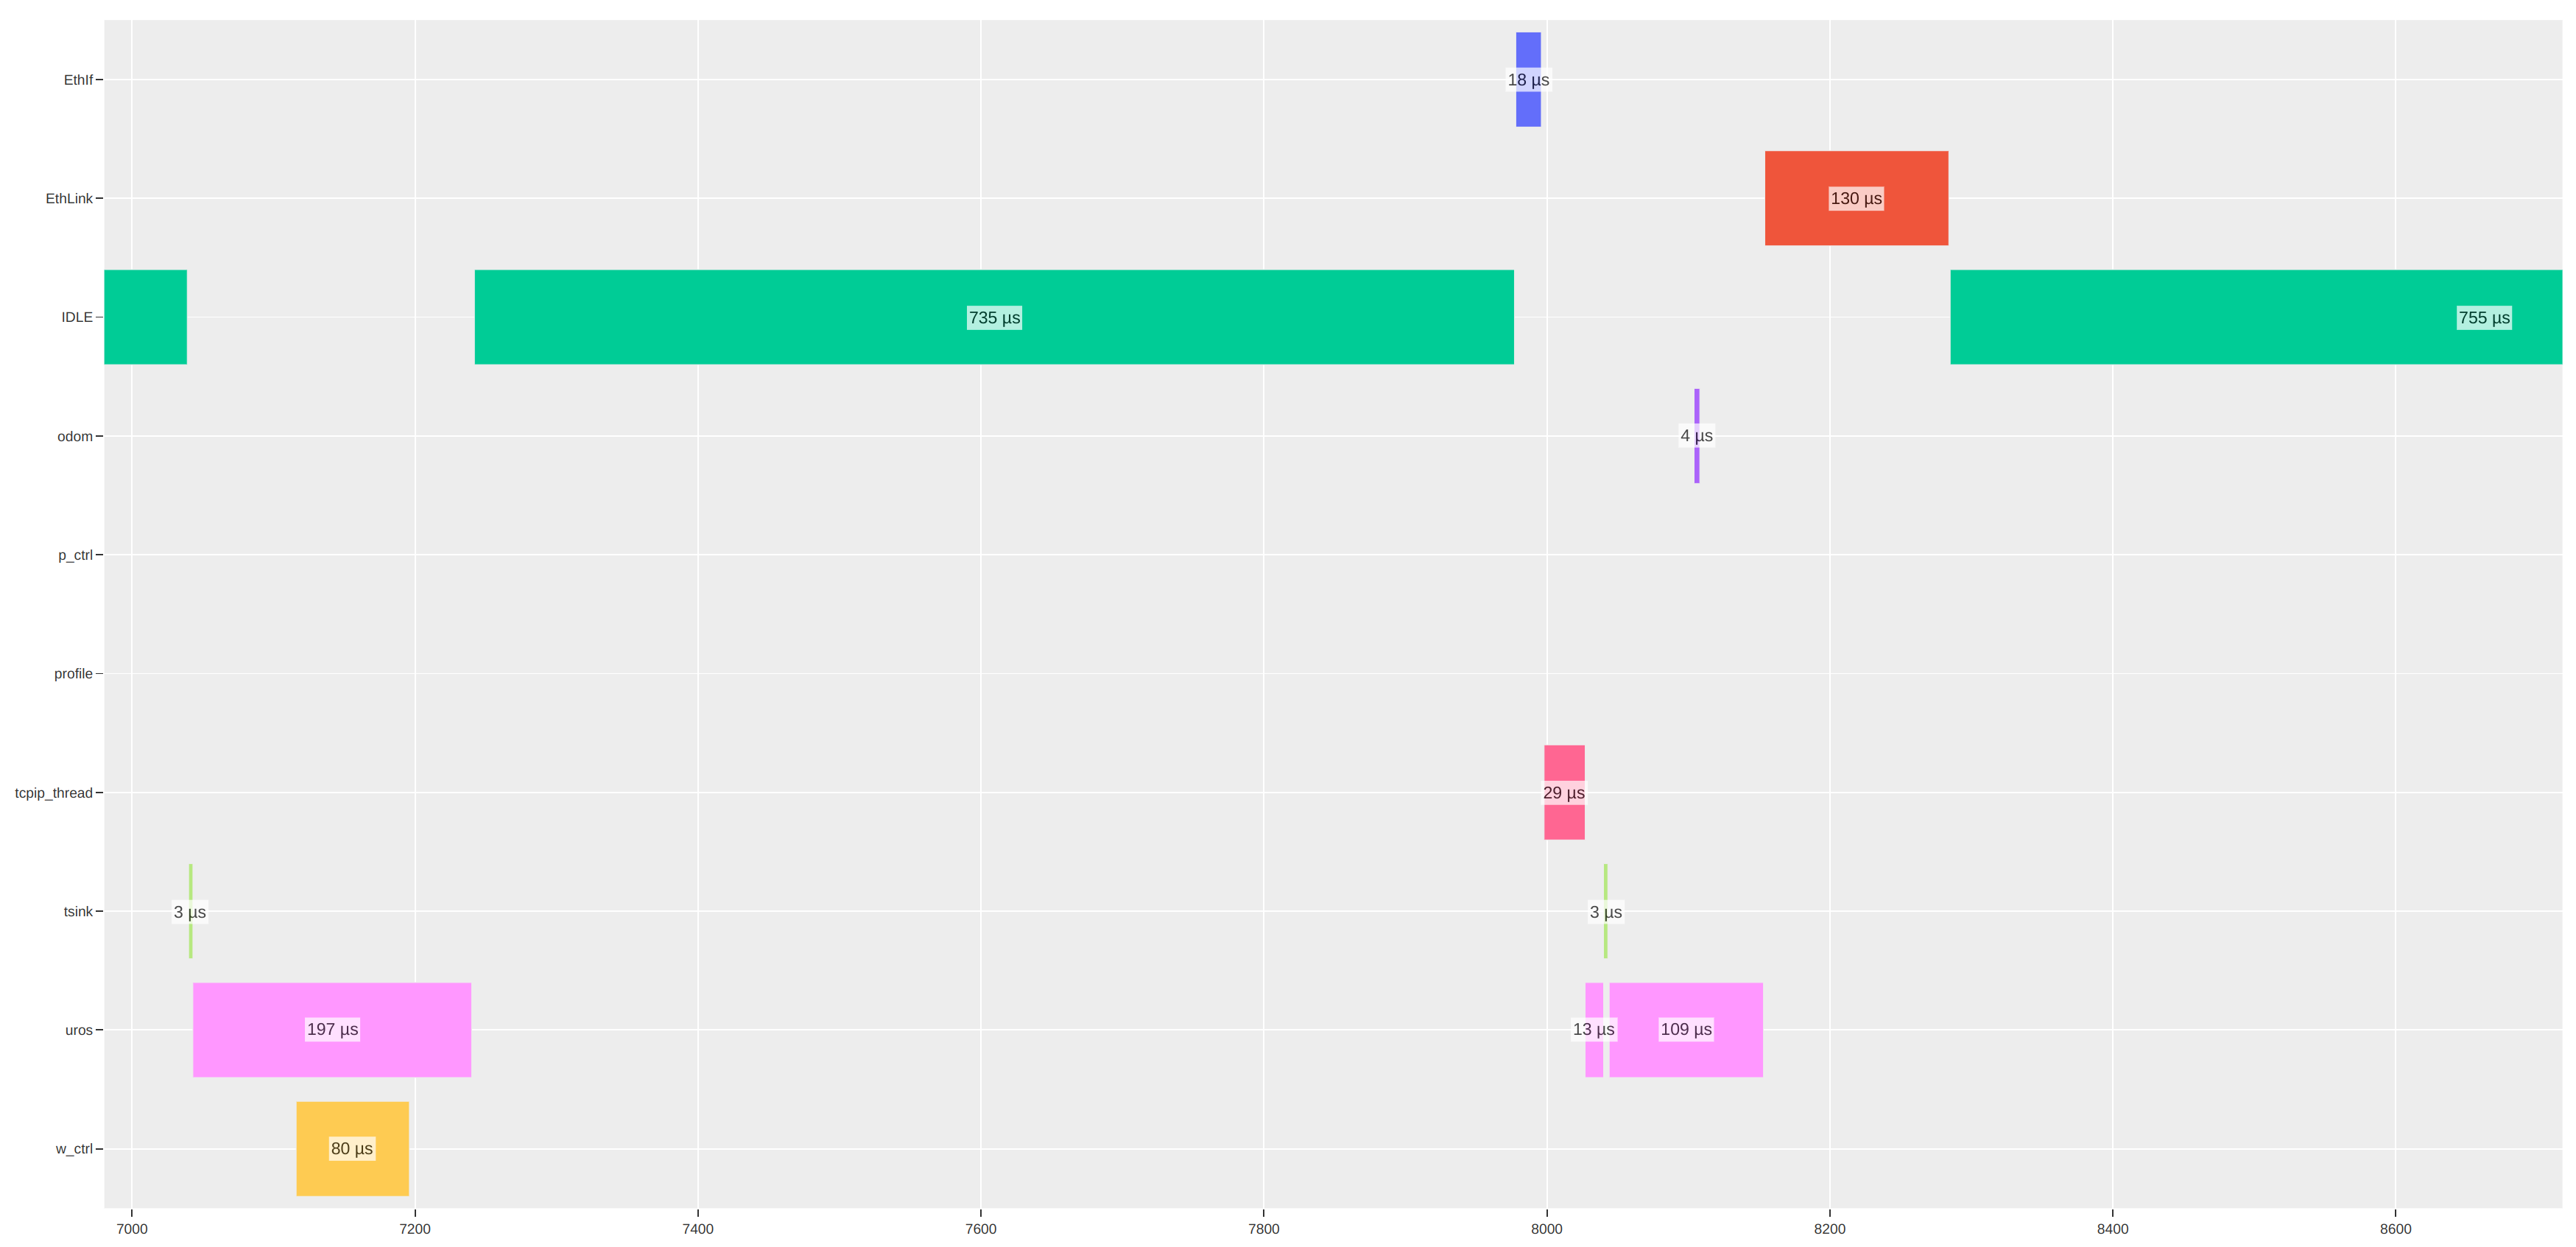
\includegraphics[width=1\textwidth]{assets/micro_ros_profiling_ausschnitt_cache_enabled}
    \caption{Echtzeitanalyse (Ausschnitt) unter Micro-ROS}
    % \label{fig:freertos_profiling}
\end{figure}

Die generierten profiling-daten reflektieren die echtzeitsaspekte bei dem
task-scheduling und den zeitkritischen funktionen. Ein Python-Skript
visualisiert diese Daten als Gantt-Diagramm, indem es die Start- und Endzeiten
mittels der \mintinline{text}|pandas| Bibliothek aggregiert, sortiert und dann
mittels der \mintinline{text}|Plotly| Bibliothek visualisiert ausgibt.

Am ende des Profilings wird eine Zusammenfassung durch von FreeRTOS
bereitgestellte \mintinline{cpp}|vTaskGetRunTimeStats()| und
\mintinline{cpp}|vTaskList()| ausgegeben.

\subsection{Laufzeit-Statistik -- Micro-ROS}

\subsubsection{Regler mit 50 Hz und 30 Hz}

Mit einer Sollfrequenz von $50\,\text{Hz}$ für die Drehzahlregelung und $30\,\text{Hz}$ für
die Posenregelung sowie Odometrie ergeben sich nach etwa $18$ Sekunden Profiling
folgende Messwerte:

\begin{table}[H]
\centering
\small
\setlength{\tabcolsep}{4pt}
\makebox[0pt][c]{\parbox{1.1\textwidth} \\ \hline
        \mintinline{text}|EthIf| & 52,93 & 115.022 & 0,62\,\% \\ \hline
        \mintinline{text}|EthLink| & 128,38 & 26.702 & 0,14\,\% \\ \hline
        \mintinline{text}|IDLE| & 587,79 & 8.961.378 & \textbf{48,17\,\%} \\ \hline
        \mintinline{text}|odom| & 8,88 & 8.186 & \textbf{0,04\,\%} \\ \hline
        \mintinline{text}|p_ctrl| & 277,97 & 170.671 & \textbf{0,92\,\%} \\ \hline
        \mintinline{text}|profile| & 623,40 & 4.981.587 & 26,78\,\% \\ \hline
        \mintinline{text}|tcpip_thread| & 71,16 & 176.607 & 0,95\,\% \\ \hline
        \mintinline{text}|tsink| & 8,80 & 120.659 & 0,65\,\% \\ \hline
        \mintinline{text}|uros| & 203,31 & 3.807.442 & \textbf{20,47\,\%} \\ \hline
        \mintinline{text}|w_ctrl| & 256,11 & 236.136 & \textbf{1,27\,\%} \\ \hline
        \hline
        \textbf{Summe} & - & 18.604.390 & 100,00\,\% \\ \hline
        \end{tabular}
        \caption{Laufzeit-Statistik ohne Caching}
    \end{minipage}
    \hfill
    \begin{minipage}[b]{0.50\hsize}\centering
        \begin{tabular}{|l|r|r|r|}
        \hline
        \textbf{Name}  & \textbf{Ø (µs)} & \textbf{Summe} & \textbf{\%} \\ \hline
        \mintinline{text}|EthIf| & 18,43 & 40.671 & 0,21\,\% \\ \hline
        \mintinline{text}|EthLink| & 123,53 & 24.583 & 0,13\,\% \\ \hline
        \mintinline{text}|IDLE| & 661,14 & 15.505.748 & \textbf{81,81\,\%} \\ \hline
        \mintinline{text}|odom| & 4,02 & 3.791 & \textbf{0,02\,\%} \\ \hline
        \mintinline{text}|p_ctrl| & 88,25 & 55.511 & \textbf{0,29\,\%} \\ \hline
        \mintinline{text}|profile| & 803,55 & 1.517.905 & 8,01\,\% \\ \hline
        \mintinline{text}|tcpip_thread| & 28,29 & 63.613 & 0,34\,\% \\ \hline
        \mintinline{text}|tsink| & 3,37 & 41.113 & 0,22\,\% \\ \hline
        \mintinline{text}|uros| & 76,17 & 1.614.854 & \textbf{8,52\,\%} \\ \hline
        \mintinline{text}|w_ctrl| & 90,82 & 85.646 & \textbf{0,45\,\%} \\ \hline
        \hline
        \textbf{Summe} & - & 18.953.435 & 100,00\,\% \\ \hline
        \end{tabular}
        \caption{Laufzeit-Statistik mit Caching}
    \end{minipage}
}}
\end{table}

\subsubsection{Regler mit 100 Hz und 50 Hz}

Mit einer Sollfrequenz von $100\,\text{Hz}$ für die Drehzahlregelung und $50\,\text{Hz}$ für
die Posenregelung sowie Odometrie ergeben sich nach etwa $18$ Sekunden Profiling
folgende Messwerte:

\begin{table}[H]
\centering
\small
\setlength{\tabcolsep}{4pt}
\makebox[0pt][c]{\parbox{1.1\textwidth} \\ \hline
        \mintinline{text}|EthIf| & 51,53 & 198.643 & 1,05\,\% \\ \hline
        \mintinline{text}|EthLink| & 110,25 & 26.130 & 0,14\,\% \\ \hline
        \mintinline{text}|IDLE| & 545,36 & 7.330.732 & \textbf{38,75\,\%} \\ \hline
        \mintinline{text}|odom| & 9,92 & 18.149 & \textbf{0,10\,\%} \\ \hline
        \mintinline{text}|p_ctrl| & 322,41 & 295.008 & \textbf{1,56\,\%} \\ \hline
        \mintinline{text}|profile| & 566,25 & 5.472.282 & 28,92\,\% \\ \hline
        \mintinline{text}|tcpip_thread| & 71,13 & 296.128 & 1,57\,\% \\ \hline
        \mintinline{text}|tsink| & 8,80 & 113.096 & 0,60\,\% \\ \hline
        \mintinline{text}|uros| & 231,74 & 4.606.256 & \textbf{24,35\,\%} \\ \hline
        \mintinline{text}|w_ctrl| & 307,53 & 562.785 & \textbf{2,97\,\%} \\ \hline
        \hline
        \textbf{Summe} & -- & 18.919.209 & 100,00\,\% \\ \hline
        \end{tabular}
        \caption{Laufzeit-Statistik ohne Caching}
    \end{minipage}
    \hfill
    \begin{minipage}[b]{0.50\hsize}\centering
        \begin{tabular}{|l|r|r|r|}
        \hline
        \textbf{Name}  & \textbf{Ø (µs)} & \textbf{Summe} & \textbf{\%} \\ \hline
        \mintinline{text}|EthIf| & 18,81 & 68.712 & 0,37\,\% \\ \hline
        \mintinline{text}|EthLink| & 128,88 & 23.971 & 0,13\,\% \\ \hline
        \mintinline{text}|IDLE| & 607,96 & 14.540.662 & \textbf{78,00\,\%} \\ \hline
        \mintinline{text}|odom| & 3,74 & 6.780 & \textbf{0,04\,\%} \\ \hline
        \mintinline{text}|p_ctrl| & 75,16 & 69.301 & \textbf{0,37\,\%} \\ \hline
        \mintinline{text}|profile| & 889,48 & 1.641.972 & 8,81\,\% \\ \hline
        \mintinline{text}|tcpip_thread| & 28,25 & 104.623 & 0,56\,\% \\ \hline
        \mintinline{text}|tsink| & 3,43 & 36.583 & 0,20\,\% \\ \hline
        \mintinline{text}|uros| & 86,44 & 1.957.616 & \textbf{10,50\,\%} \\ \hline
        \mintinline{text}|w_ctrl| & 103,59 & 191.027 & \textbf{1,02\,\%} \\ \hline
        \hline
        \textbf{Summe} & -- & 18.641.247 & 100,00\,\% \\ \hline
        \end{tabular}
        \caption{Laufzeit-Statistik mit Caching}
    \end{minipage}
}}
\end{table}

Ohne D- oder I-Cache benötigte die Micro-ROS-Task (\mintinline{text}|uros|) für
die gesamte Steuerungslogik bei den Reglern mit jeweils $50$ und $30\,\text{Hz}$
$\textbf{20,47\,\%}$ Rechenzeit, bzw. $\textbf{24,35\,\%}$ bei jeweils $100$ und
$50\,\text{Hz}$, während sich das System zu $\textbf{48,17\,\%}$ bzw.
$\textbf{38,75\,\%}$ im Leerlauf befindet.

Mit dem D- und I-Cache benötigt die Robotersteuerungslogik insgesamt nur
$\textbf{8,52\,\%}$ Rechenzeit bei den Reglern mit jeweils $50$ und
$30\,\text{Hz}$, oder $\textbf{10,50\,\%}$ bei jeweils $100$ und
$50\,\text{Hz}$, mit einer Leerlaufzeit von $\textbf{81,81\,\%}$ oder
$\textbf{78,00\,\%}.$

Durch das Aktivieren von Caches hat sich die akkumulierte Rechenzeit
beispielsweise bei der $100\,\text{Hz}|50\,\text{Hz}$ Regler-Konfiguration für
die Odometrie um $\textbf{62,64\,\%},$ für die Posenregelung um
$\textbf{76,51\,\%}$ sowie für die Drehzahlregelung um $\textbf{66,06\,\%}$
verringert, während die Leerlaufzeiten um $\textbf{98,35\,\%}$ erhöht wurden,
wobei sich die gesamten Profiling-Dauer mit einer Differenz von
$349,045\,\text{ms}$ unterscheiden.

\subsection{Laufzeit-Statistik -- FreeRTOS}

\subsubsection{Regler mit 50 Hz und 30 Hz}

\begin{table}[H]
\centering
\small
\setlength{\tabcolsep}{4pt}
\makebox[0pt][c]{\parbox{1.1\textwidth} \\ \hline
        \mintinline{text}|IDLE| & 983,50 & 14.996.422 & \textbf{81,85\%} \\ \hline
        \mintinline{text}|hal_fetch| & 21,71 & 20.403 & 0,11\% \\ \hline
        \mintinline{text}|odometry| & 24,05 & 13.634 & \textbf{0,07\%} \\ \hline
        \mintinline{text}|pose_control| & 32,66 & 18.682 & \textbf{0,10\%} \\ \hline
        \mintinline{text}|profile| & 902,87 & 3.077.879 & 16,80\% \\ \hline
        \mintinline{text}|tsink| & 9,63 & 161.451 & 0,88\% \\ \hline
        \mintinline{text}|wheel_ctrl| & 35,80 & 34.260 & \textbf{0,19\%} \\ \hline
        \hline
        \textbf{Summe} & -- & 18.322.731 & 100,00\,\% \\ \hline
        \end{tabular}
        \caption{Laufzeit-Statistik ohne Caching}
    \end{minipage}
    \hfill
    \begin{minipage}[b]{0.50\hsize}\centering
        \begin{tabular}{|l|r|r|r|}
        \hline
        \textbf{Name}  & \textbf{Ø (µs)} & \textbf{Summe} & \textbf{\%} \\ \hline
        \mintinline{text}|IDLE| & 1.041,06 & 17.658.382 & \textbf{94,83\,\%} \\ \hline
        \mintinline{text}|hal_fetch| & 6,43 & 6.003 & 0,03\,\% \\ \hline
        \mintinline{text}|odometry| & 7,19 & 4.068 & \textbf{0,02\,\%} \\ \hline
        \mintinline{text}|pose_control| & 9,64 & 5.456 & \textbf{0,03\,\%} \\ \hline
        \mintinline{text}|profile| & 476,43 & 889.027 & 4,77\,\% \\ \hline
        \mintinline{text}|tsink| & 2,95 & 46.947 & 0,25\,\% \\ \hline
        \mintinline{text}|wheel_ctrl| & 10,96 & 10.379 & \textbf{0,06\,\%} \\ \hline
        \hline
        \textbf{Summe} & -- & 18.620.262 & 100,00\,\% \\ \hline
        \end{tabular}
        \caption{Laufzeit-Statistik mit Caching}
    \end{minipage}
}}
\end{table}

\subsubsection{Regler mit 100 Hz und 50 Hz}

\begin{table}[H]
\centering
\small
\setlength{\tabcolsep}{4pt}
\makebox[0pt][c]{\parbox{1.1\textwidth} \\ \hline
        \mintinline{text}|IDLE| & 997,02 & 14.706.086 & \textbf{80,67\,\%} \\ \hline
        \mintinline{text}|hal_fetch| & 21,91 & 40.471 & 0,22\,\% \\ \hline
        \mintinline{text}|odometry| & 24,01 & 22.373 & \textbf{0,12\,\%} \\ \hline
        \mintinline{text}|pose_control| & 32,46 & 30.579 & \textbf{0,17\,\%} \\ \hline
        \mintinline{text}|profile| & 941,93 & 3.209.167 & 17,60\,\% \\ \hline
        \mintinline{text}|tsink| & 9,36 & 151.046 & 0,83\,\% \\ \hline
        \mintinline{text}|wheel_ctrl| & 37,77 & 70.285 & \textbf{0,39\,\%} \\ \hline
        \hline
        \textbf{Summe} & {--} & 18.230.007 & 100,00\,\% \\ \hline
        \end{tabular}
        \caption{Laufzeit-Statistik ohne Caching}
    \end{minipage}
    \hfill
    \begin{minipage}[b]{0.50\hsize}\centering
        \begin{tabular}{|l|r|r|r|}
        \hline
        \textbf{Name}  & \textbf{Ø (µs)} & \textbf{Summe} & \textbf{\%} \\ \hline
        \mintinline{text}|IDLE| & 1.139,87 & 17.276.974 & \textbf{94,61\,\%} \\ \hline
        \mintinline{text}|hal_fetch| & 6,61 & 12.104 & 0,07\,\% \\ \hline
        \mintinline{text}|odometry| & 6,84 & 6.256 & \textbf{0,03\,\%} \\ \hline
        \mintinline{text}|pose_control| & 9,88 & 9.043 & \textbf{0,05\,\%} \\ \hline
        \mintinline{text}|profile| & 487,57 & 892.246 & 4,89\,\% \\ \hline
        \mintinline{text}|tsink| & 3,01 & 45.597 & 0,25\,\% \\ \hline
        \mintinline{text}|wheel_ctrl| & 10,69 & 19.559 & \textbf{0,11\,\%} \\ \hline
        \hline
        \textbf{Summe} & {--} & 18.443.591 & 100.00\,\% \\ \hline
        \end{tabular}
        \caption{Laufzeit-Statistik mit Caching}
    \end{minipage}
}}
\end{table}

Ohne die Micro-ROS-Abhängigkeit erreicht das System bereits ohne Nutzung von
Caches eine Leerlaufzeit von circa $\textbf{80\,\%}$, und mit Nutzung von Caches
von circa $\textbf{95\,\%}$.

Die Performance-Steigerung durch das Aktivieren der Caches ist bei der
FreeRTOS-Implementierung ebenfalls signifikant, wobei sich die gesamten
Profiling-Dauer bei der $100\,\text{Hz}|50\,\text{Hz}$-Reglerkonfiguration um
$213,584\,\text{ms}$ unterscheiden. Die Leerlaufzeit stieg dadurch zwar nur um
$\textbf{14,88\,\%}$, jedoch verringerten sich die Rechenzeiten deutlich: für
die Odometrie um $\textbf{72,04\,\%}$, für die Posenregelung um
$\textbf{70,43\,\%}$ und für die Drehzahlregelung um $\textbf{72,17\,\%}$.

\subsection{Vergleich zwischen Micro-ROS und FreeRTOS}

% | name | unter Micro-ROS (µs) | unter FreeRTOS (µs) | Differenz (µs) |
% | Odometrie | 6.780 (Ø: 3,74) | 6.256 (Ø: 6,84) | -524 |
% | Posenregelung | 69.301 (Ø: 75,16) | 9043 (Ø: 9,88) | 60258 (Ø: 65,28) |
% | Drehzahlregelung |191.027 (Ø: 103,59) | 19.559 (Ø: 10,69) | 171468 (Ø: 92,90) |

Aus den Profiling-Daten lässt sich folgender Vergleich zwischen der Micro-ROS-
und FreeRTOS-Implementierung für die Robotersteuerung ableiten:

\begin{table}[h]
\centering
\begin{tabular}{|l|r|r|r|}
\hline
    \textbf{Name} & \textbf{Micro-ROS (\text{µs})} & \textbf{FreeRTOS (\text{µs})} & \textbf{Differenz (\text{µs})} \\ \hline
Odometrie & 6.780 (Ø:~3,74) & 6.256 (Ø:~6,84) & -524 \\ \hline
Posenregelung & 69.301 (Ø:~75,16) & 9.043 (Ø:~9,88) & 60.258 (Ø:~65,28) \\ \hline
Drehzahlregelung & 191.027 (Ø:~103,59) & 19.559 (Ø:~10,69) & 171.468 (Ø:~92,90) \\ \hline
\end{tabular}
\caption{Vergleich der Rechenzeiten zwischen Micro-ROS und FreeRTOS}
\end{table}

Die Implementierung bleibt auf beiden Plattformen größtenteils gleich, abgesehen
vom Datenaustausch. Bei Micro-ROS müssen die Daten zusätzlich in einer
dedizierten Struktur mit Metadaten -- unter anderem einem Header mit Zeitstempel
in Sekunden und Nanosekunden -- umgewandelt werden, was einen wesentlichen
Overhead im Vergleich zu FreeRTOS verursacht. Dort können die Daten als
einfache, array-ähnliche Struktur direkt in die Warteschlange kopiert und
extrahiert werden.

Zusätzlich unterscheidet sich die FreeRTOS-Implementierung von Micro-ROS
dadurch, dass die Drehzahldaten nicht direkt vom Drehzahlregler abgefragt und an
die Odometrie übergeben werden. Stattdessen übernimmt eine dedizierte
FreeRTOS-Task \mintinline{cpp}|hal_fetch| die Übertragung dieser Daten sowohl an
den Drehzahlregler als auch an die Odometrie. Dadurch wird ein Teil des
Overheads vom Drehzahlregler entkoppelt.

Zusammenfassend lässt sich feststellen, dass die Robotersteuerungslogik sowohl
unter Micro-ROS als auch unter FreeRTOS vergleichsweise wenig Rechenzeit
benötigt. Dies gilt selbst bei potenziell höheren Sollfrequenzen, sofern die
Daten gecacht sind und nicht bei jedem Zugriff aus dem RAM geladen werden
müssen, welcher wesentlich langsamer ist als der L1-Cache. Dank des
leistungsstarken Mikrocontrollers in Kombination mit Cache-Nutzung und
optimiertem Code befindet sich das System daher überwiegend im Leerlauf.

\newpage

\section{Zusammenfassung}

Am Anfang wurde die Robotersteuerungssoftware von Micro-ROS auf FreeRTOS
umgestellt. Anschließend wurden eine Multi-Producer-Senke sowie ein Verfahren
entwickelt, das Laufzeitinformationen über die Steuerungssoftware ausgeben kann.
Abschließend wurde die Echtzeitfähigkeit basierend auf die erzeugten
Laufzeitdaten analysiert.

Es lässt sich schlussfolgern, dass die Steuerungssoftware zwar durch Integration
von Micro-ROS funktionsreicher und folglich mit einer Vielzahl von
ROS-Komponenten kompatibel wird, dies allerdings mit erheblichem Overhead
erkauft wird. Bei begrenztem Speicher oder Rechenleistung bleibt FreeRTOS mit
seinem schlanken Kernel und den standardmäßig threadsicheren Queue-Abstraktionen
weiterhin eine geeignete Wahl gegenüber komplexeren RTOS-Lösungen --
insbesondere wenn hochfrequente Aufgabenausführungen mit Echtzeitanforderungen
prioritär sind.

Zudem wurde demonstriert, dass L1-Caches die Performance signifikant steigern --
eine für leistungskritische Software wesentliche Optimierung, die nicht
vernachlässigt werden darf.

Für zukünftige Arbeiten könnte die Multi-Producer-Senke so weiterentwickelt
werden, dass sie Schreiboperationen atomar auf 4-Byte-/32-Bit-Ebene unterstützt.
Dadurch könnten die Laufzeitdaten nicht mehr im menschenlesbaren Format mit
überflüssigem Daten-Overhead, sondern komprimiert jeweils als 32-Bit-Datenwort
ausgegeben werden.

Dies würde erstens den Zwischenpuffer und den erforderlichen Mutex zum
Serialisieren sowie Speichern von erzeugten Laufzeitdaten überflüssig machen, da
sie als 32-bit-Datenworte atomar direkt in die Senke geschrieben werden könnten.
Zweitens könnte dann ein dedizierter Parser auf dem Linux-Host entwickelt
werden, der die Visualisierung übernimmt und idealerweise eine Echtzeitanalyse
parallel zur Laufzeit durchführt.

% Diese Vorgehensweise ähnelt der Rust-Bibliothek \mintinline{text}|defmt|, bei
% der die rechenintensive Formatierung von Logging-Informationen nicht auf dem
% ressourcenbeschränkten System erfolgt, sondern auf eine sekundäre Maschine
% ausgelagert wird.

\newpage

\pagenumbering{Roman}
% einfacher Zeilenabstand
\singlespacing
% Literaturliste soll im Inhaltsverzeichnis auftauchen
\newpage
\phantomsection
\addcontentsline{toc}{section}{Literaturverzeichnis}
% Literaturverzeichnis anzeigen
\renewcommand\refname{Literaturverzeichnis}
\bibliography{Hauptdatei}

%% Index soll Stichwortverzeichnis heissen
% \newpage
% % Stichwortverzeichnis soll im Inhaltsverzeichnis auftauchen
% \addcontentsline{toc}{section}{Stichwortverzeichnis}
% \renewcommand{\indexname}{Stichwortverzeichnis}
% % Stichwortverzeichnis endgültig anzeigen
% \printindex

% \onehalfspacing
% % evtl. Anhang
% \newpage
% \phantomsection
% \addcontentsline{toc}{section}{Anhang}
% \fancyhead[L]{Anhang} %Kopfzeile links
% \input{anhang}

% \newpage
% \includepdf[pages=1, fitpaper=true]{flattened.pdf}

% \fancyhead[L]{Eigenständigkeitserklährung} %Kopfzeile links
% \input{eigenstaendigkeitserklaehrung} % deleted 

\end{document}
